\documentclass[12pt,letterpaper]{lsuetd}
\usepackage{setspace,graphics,dsfont,verbatim,paralist,indentfirst,amsmath,amssymb}
\setlength{\topmargin}{-0.5in}
\setlength{\textheight}{9.0in}
\addtolength{\evensidemargin}{-0.50in}
\addtolength{\oddsidemargin}{-0.50in}
\addtolength{\textwidth}{1.00in}
\setlength{\parindent}{1.75em}
\setlength{\parskip}{0ex}
\setcounter{tocdepth}{2}

\makeatletter

\begin{document}
\renewcommand\@pnumwidth{1.55em}
\renewcommand\@tocrmarg{9.55em}
\renewcommand*\l@chapter{\@dottedtocline{0}{1.5em}{2.3em}}
\renewcommand*\l@figure{\@dottedtocline{1}{0em}{3.1em}}
\let\l@table\l@figure

\pagenumbering{roman}
\thispagestyle{empty}
\begin{center}
%The title page is first created.
  STRATEGIES FOR COMPUTING THE SCALAR SELF-FORCE ON A SCHWARSZCHILD BACKGROUND: A COMPARISON STUDY WITH AN FORTRAN CODE IN C++, EXTRAPOLATING TO INFINITE DISCONTINUOUS GALERKIN ORDER, AND EXTRAPOLATING TO INFINITE SPHERICAL HARMONIC MODES

\vfill
\doublespacing
A Thesis/Dissertation \\
\singlespacing
Submitted to the Graduate Faculty of the \\
Louisiana State University and \\
Agricultural and Mechanical College \\
in partial fulfillment of the \\
requirements for the degree of \\
Master of Science\\
\doublespacing
in \\
                                       
Physics\\
\singlespacing
\vfill

by \\
Steven (Susan) Dorsher \\
B.S., Massachusetts Institute of Technology, 2004  \\
M.S., The Ohio State University, 2006  \\
M.S., University of Minnesota, 2013  \\
%If necessary, copy and paste the previous line here to include a master's degree.
December, 2017
\end{center}
\pagebreak
%The Copyright Page and Dedication sections can be added here, if desired.

%\chapter*{Copyright Page}
%\doublespacing
%\vspace{0.55ex}
%Insert the appropriate text for the copyright page here.
%\addcontentsline{toc}{chapter}{\hspace{-1.5em} {COPYRIGHT PAGE} \vspace{12pt}}
%\pagebreak

%\chapter*{Dedication}
%\doublespacing
%\vspace{0.55ex}
%Insert the appropriate text for the dedication or epigraph page here.  This part of the ETD must not exceed one page.
%\addcontentsline{toc}{chapter}{\hspace{-1.5em} {DEDICATION} \vspace{12pt}}
%\pagebreak

\chapter*{Acknowledgments}
\doublespacing
\vspace{0.55ex}
I would like to thank Peter Diener and Frank L\"{o}ffler for their guidance. Peter Diener especially has been very important to me, both as an advisor and personally. I would also like to thank Gabriela Gonzalez for the excellent opportunity to work on LIGO during the time of three detections, which provided me the funding I needed to continue the work detailed in this document. I would like to thank Juana Moreno for the opportunity to work as outreach coordinator to the LA-SIGMA Research Experience for Undergraduates program my first summer at LSU, which also helped provide funding for this research. My parents, Paul and Joanne Dorsher, also deserve a mention, both for extraordinary moral support and for the financial support they provided that helped make this possible. I would also like to thank my sister Patricia Dorsher, my grandmother Evie Dorsher and her sister Gwen Helbling, and my Aunt Peggy Bennett, and my Aunt Elaine Shirley for being my anchor. I would like to thank my friends Christy Paulson, Hope Ring, Steve Brandt, Brad Schaefer, Luke, and Josh McKeown for their company and kindness during this process. My family, friends, and loved ones are the purpose behind this work. 

%The code below adds the Acknowledgments section to the Table of Contents.
\addcontentsline{toc}{chapter}{\hspace{-1.5em} {ACKNOWLEDGMENTS} \vspace{12pt}}
\pagebreak
%The Preface section can now be added, if desired.

%\chapter*{Preface}
%\doublespacing
%\vspace{0.55ex}
%Insert the appropriate text for the preface here.
%\addcontentsline{toc}{chapter}{\hspace{-1.5em} {PREFACE} \vspace{12pt}}
%\pagebreak

\singlespacing
\tableofcontents
\pagebreak

%The code below generates the List of Tables and adds it to the Table of Contents.
\renewcommand\@pnumwidth{1.55em}
\renewcommand\@tocrmarg{8.55em}
\addcontentsline{toc}{chapter}{\hspace{-1.5em} LIST OF TABLES \vspace{12pt}}
\listoftables
\pagebreak
%The code below generates the List of Figures and adds it to the Table of Contents.
\addcontentsline{toc}{chapter}{\hspace{-1.5em} LIST OF FIGURES \vspace{12pt}}
\listoffigures
\pagebreak
%The List of Nomenclature may be included here, if desired.

%\chapter*{List of Nomenclature}
%\doublespacing
%\vspace{0.55ex}
%Provide the definitions of the symbols used in your thesis or dissertation here.
%\addcontentsline{toc}{chapter}{\hspace{-1.5em} LIST OF NOMENCLATURE \vspace{12pt}}
%\pagebreak

%The code below adds the Abstract and places it within the Table of Contents.
\renewenvironment{abstract}{{\hspace{-2.2em} \huge \textbf{\abstractname}} \par}{\pagebreak}
\addcontentsline{toc}{chapter}{\hspace{-1.5em} ABSTRACT}
\begin{abstract}
\vspace{0.55ex}
\doublespacing
Insert the text of your abstract here.  Make sure there is one blank line between the end of the Abstract text and the ``end'' command below to maintain double--spaced lines.

\end{abstract}

\pagenumbering{arabic}
\addtocontents{toc}{\vspace{12pt} \hspace{-1.8em} CHAPTER \vspace{-1em}}
\singlespacing
\setlength{\textfloatsep}{12pt plus 2pt minus 2pt}
\setlength{\intextsep}{6pt plus 2pt minus 2pt}
\chapter{Introduction}
\doublespacing
\section{Gravitational Waves}

On February 11, 2016, the LIGO Scientific Collaboration announced the
first detection of gravitational waves from a black hole binary
inspirals, occurring on September 14, 2015, with pre-merger masses of
36 $M_\odot$ and 29 $M_\odot$ and a post merger mass of 62 $M_\odot$
at a redshift of $z=0.09$~\cite{GW150914}. Two subsequent detections
followed, on December 26, 2015~\cite{GW151226} and on January 4,
2017~\cite{GW170104}, with masses that are about the same to within an order of magnitude.

There is a question of what is meant, observationally, by a black hole. Does it need to have a horizon? Does it need to have a Kerr metric (the simplest possible space-time for a spinning black hole in general relativity)? Does it simply need to be a sufficiently compact object that it can't be ordinary nuclear matter? Historically, black holes have been defined by their compactness~\cite{Bambi2017}; however, some studies are beginning to consider tests of horizons~\cite{} or of the Kerr metric itself~\cite{Bambi2017}. X-ray binaries, gravitational wave constraints from binary-pulsar systems, active galactic nucleii models containing super-massive black holes on the order of $10^6 M_\odot$, and the three LIGO detections, as well as black hole formation models, suggest that black holes of all scales should be spinning~\cite{Bambi2017}. However, for the purposes of this manuscript, I will consider non-spinning, spherically symmetric black holes in general relativity, described by the Schwarzschild metric.

Currently, there are four distinct windows on the gravitational wave universe planned or in progress. The Laser Interferometer Gravitational Wave Observatory, LIGO, probably deserves first listing, due to their recent success. LIGO observes gravitational waves using a ground based Michelson-Morley interferometer with two 4 kilometer long Fabry-Perot cavity arms. It detects strains as small as $10^-{23} Hz^{-1/2}$~\cite{LIGOsensitivity}.

\begin{figure}
  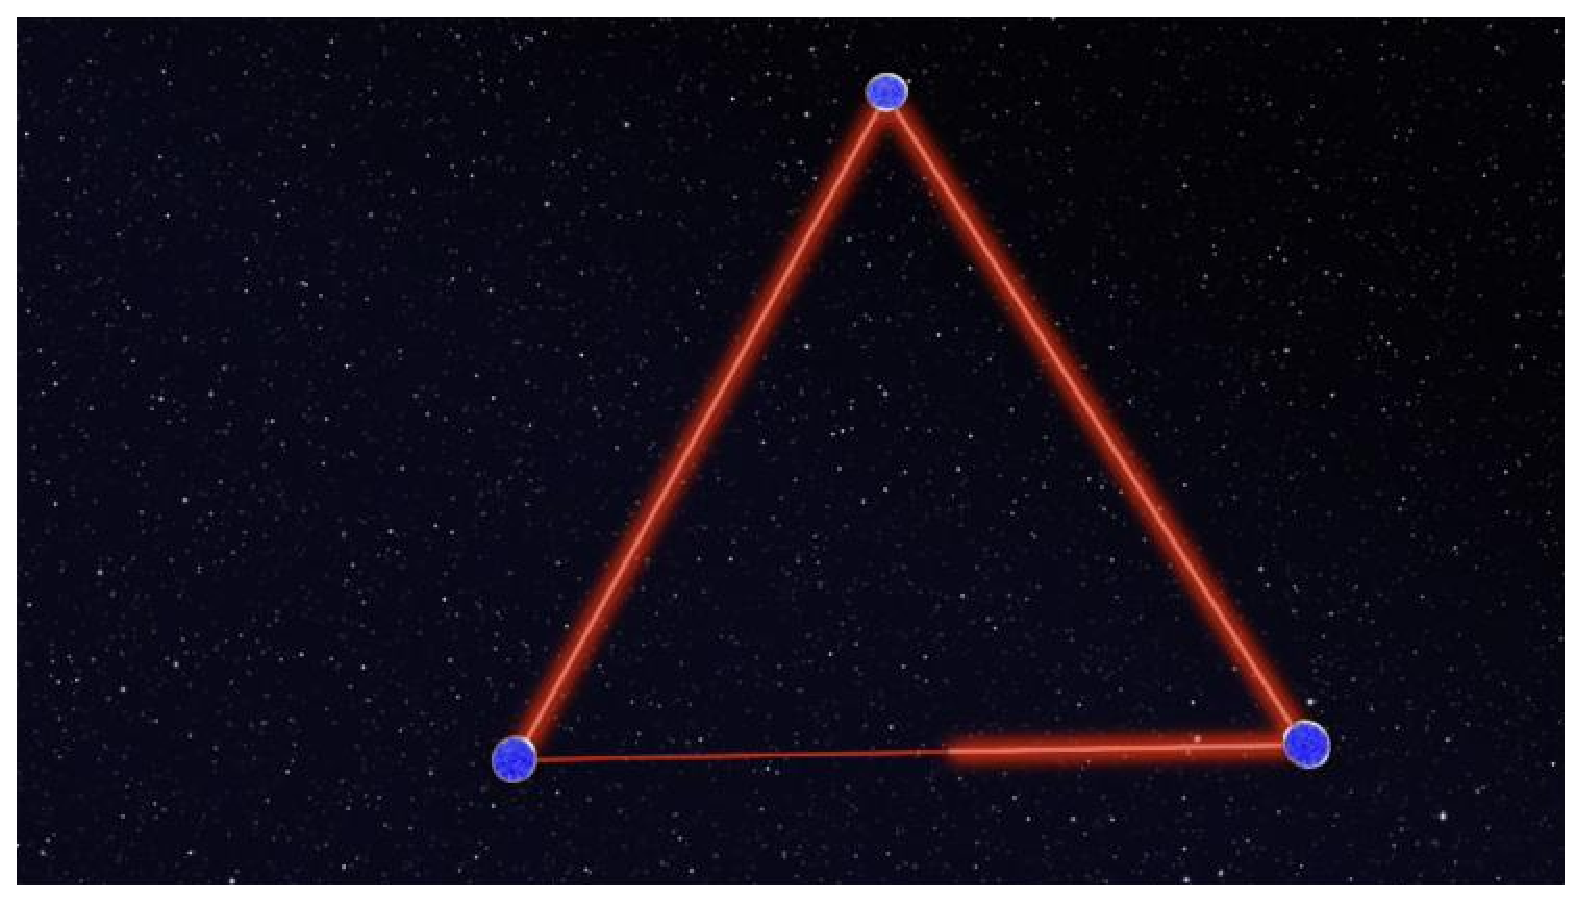
\includegraphics{eLISA}
\end{figure}

\begin{figure}
  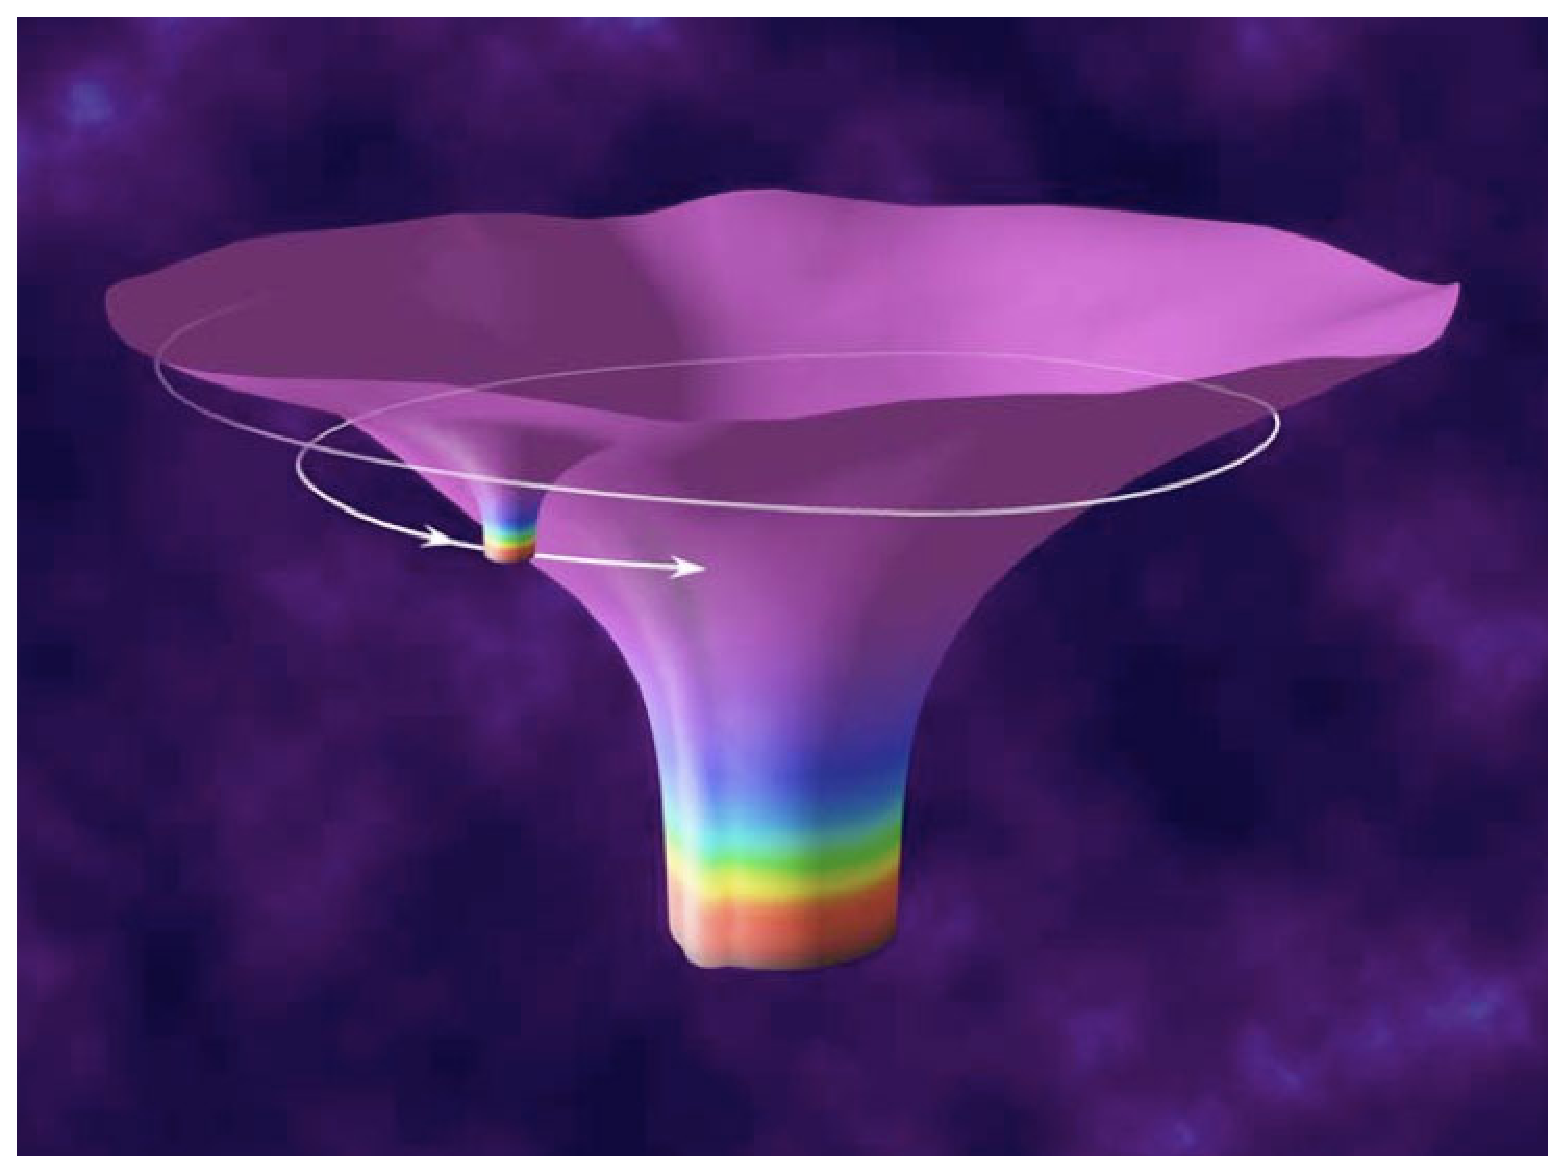
\includegraphics{EMRI}
\end{figure}



%Thornberg
%Warburton
%Wardell
%Diener
%adam pound
%bernard whiting
%ian vega
%anna hesthaven
%maarten van de meent
%jonathan thompson
%jordan moxon?

\section{Extreme Mass Ratio Inspirals}

\section{EMRIs}
\section{The discontinuous galerkin method}
\section{LISA}

\pagebreak
\singlespacing
\chapter{A simple numerical solution for a PDE using the Discontinuous Galerkin method}
\doublespacing
\section{Reduction to coupled first order differential equations}


The fundamental problem we wish to solve is to evolve the wave equation on Schwarzschild space-time with a source. However, to begin to address this problem, I implemented a one dimensional wave equation solver in C++ using the Discontinuous Galerkin method in flat space-time. The wave equation in flat space-time is given, in several different forms, by
\begin{eqnarray}
  \Box\psi=0\\
  \frac{\partial^2\psi}{\partial t^2}=\nabla\psi\\
  \frac{\partial^2\psi}{\partial t^2}=\frac{\partial^2 \psi}{\partial r^2}
\end{eqnarray}
where the final form is specialized to one dimension and $c=1$ in natural units. To numerically integrate this, it is necessary to reduce this second order differential equation to three coupled differential first order differential equations. There is a classical solution to this problem, which we follow. We introduce variables $\rho=\frac{\partial \psi}{\partial t}$ and $\phi = \frac{\partial\psi}{\partial r}$. With these definitions, and remembering that we want time evolution equations rather than spatial evolution equations, the three coupled equations become
\begin{eqnarray}
  \frac{\partial\psi}{\partial t} = \rho\nonumber\\
  \frac{\partial\rho}{\partial t} = \frac{\partial \phi}{\partial r}\nonumber\\
  \frac{\partial\phi}{\partial t} = \frac{\partial \rho}{\partial r}
  \label{stateev}
\end{eqnarray}
This system of equations can be rewritten
\begin{equation}
  \frac{\partial u}{\partial t} = A\frac{\partial u}{\partial r} + Bu\nonumber\\
  \frac{\partial u}{\partial t} = RHS(u,t)
  \label{matrixdiff}
\end{equation}
where $u$ is the state vector consisting of $u=(\psi,\rho,\phi)$, and $A$ and $B$ are matrices. RHS stands for Right Hand Side. The C++ code has been implemented for wave equations of this generalized form, which encompasses wave equations on a Schwarzschild space-time.




\section{Spatial grids}
Our code solves a wave equation, which must first calculate a spatial derivative then integrate in time to solve a differential equation. For the spatial derivative part of the scheme, we make use of the Discontinuous Galerkin method to compute spatial derivatives, as a replacement for a finite difference scheme. Its has three primary benefits. One is that it naturally handles discontinuities in the evolved field, which is important to the effective source approach that we use when calculating orbits with a source in curved space-time. The second is that its accuracy scales exponentially with increasing polynomial order. 


\subsection{Finite difference schemes}
The classic solution to the spatial derivative problem is the finite difference scheme. In a one dimensional finite difference scheme, space is discretized into points on a line. The spatial derivative is calculated using a stencil of points that is symmetric about the point where one wants to know the spatial derivative, and extends $2n$ points beyond to either side, where $n$ is the order of the expansion. The spatial derivative is calculated from a weighted sum of the points included in the stencil, where some of the weights are negative. A stencil with $2n-1$ points in it, in one dimension, corresponds to an $n$th order expansion. It is possible to expand any order of derivative to any order of expansion. A first derivative, to second order accuracy, given by:
\begin{equation}
  D_r^{(2)}=\frac{1}{h}(-\frac{1}{2}f_{-1}+\frac{1}{2}f_1)
\end{equation}
Here the $f_{-1}$ and $f_1$ indicate the function evaluated at the grid point to either side of the $0$th grid point, where the derivative is evaluated. Here $h$ is the spacing between grid points. 
\begin{equation}
  D_r^{\prime (2)}=\frac{1}{h^2}(f_{-1}-2f_0+f_1)
\end{equation}

It is possible to extend these stencils to two and three dimensions. When considering parallelization using OpenMP, issues of synchronization must be considered. When parallelizing over many nodes, the spatial grid gets divided into blocks. At the ends of each block, the boundary cells need information from the neighboring cells to calculate the spatial derivative. For an order $n$ derivative, $n-1$ boundary cells are synchronized into buffer zones both to the left and to the right at each time step. In our code, this is not necessary, since we have parallelized with OpenMP, which uses shared memory within one node, across several (16) cores.

\subsection{The Discontinuous Galerkin method}
The Discontinuous Galerkin method breaks space into segments called elements. Within each element, the value of the field is represented by the sum of $n+1$ interpolating polynomials of order $n$, where $n$ is the order of the element. There are $n+1$ unevenly spaced nodes in the element, clustered toward the edges. At each node, exactly one of the interpolating polynomials takes on a value of one while the others are zero. An interpolating Lagrange polynomial has a functional form:
\begin{equation}
  \ell_i(r)=\prod_{j=1,j\ne i}^{n}\frac{r-\xi_j}{\xi_i-\xi_j}
\end{equation}
where $\xi_i$ is a location of a node and where $r$ is an arbitrary position~\cite{dghesthaven}. 


Omitting the details of the derivation of this method, which can be found in Reference~\cite{dghesthaven}, the procedure for calculating the spatial derivative in one dimension is to first calculate the Legendre polynomials. A matrix inversion is involved to calculate the derivative matrices, for which we use custom packages, the Template Numerical Toolkit and JAMA. It was discovered, upon parallelization with OpenMP, that TNT is not threadsafe. I rewrote most, but not all, of the code to avoid this issue; however, it would be better to replace TNT altogether if this code were developed further.

The Discontinuous Galerkin method helps damp error introduced by discontinuities in the field, provided they remain at element boundaries. We make use of this in our self-force calculations in the neighborhood of the particle, to be described in Chapter~\ref{ellipticalorb}. The numerical flux how information passes from one element to the next in the Discontinuous Galerkin method and is a way of accounting for the discontinuity in the flow between neighboring elements. The specific method we use for calculating the numerical flux breaks breaks the wave velocities into in-going and outgoing components. At each element boundary, the state vector from external to the element is coupled to the in-going velocity then added to the state vector internal to the element coupled to the outgoing velocity. The contribution from each boundary is distributed across the element according to a lift matrix. This is repeated at each time step. Discontinuities can exist at the boundaries, but not within an element. 



\section{Time evolution}

Time evolution in our code is handled by a fourth order low storage Runga Kutta method. Instead of the standard fourth order Runga Kutta method, this method takes five sub-time-steps, but only the most recent sub-time-step needs to be stored.

\begin{eqnarray}
  p^{(0)}=&u^n\nonumbuer\\
  k^{(i)}=&a_ik^{(i-1)}+\delta t RHS(p^{(i-1)},t^n+c_i\delta t)\nonumber\\
  p^{(i)}=&p^{(i-1)}+b_iK^{(i)}\nonumber\\
  u_h^{n+1}=&p^{(5)}
\end{eqnarray}
Here steps two and three are repeated for $i=1-5$, first $k$, then $p$, then increase $i$ and repeat. The coefficients $a_i$, $b_i$, and $c_i$ are given in Reference~\cite{dghesthaven}.

\section{Wave equation on flat space-time}

Using Gaussian initial conditions in $\psi$ and setting the $\rho$ (Equation~\ref{statev}) initial conditions to the derivative of that Gaussian, I have produced the evolution shown in Figure~\ref{gaussWave}. The Gaussian splits into two, evolves both left and right, hits the periodic boundary conditions, and re-enters the one-dimensional space on the opposite side, eventually returning to its original position and re-merging. A progression from left to right can be seen in Figure~\ref{sineWave} for sinusoidal initial conditions with a sinusoidal initial condition in $\psi$ and cosine initial conditions in $\phi$ (Equation~\ref{stateev}). Again, periodic boundary conditions cause the wave to cross to the opposite side and re-enter.

\begin{figure}
  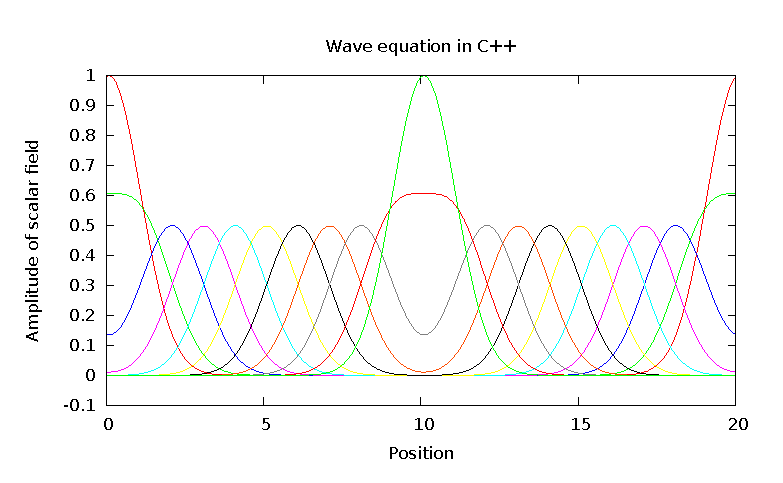
\includegraphics{gaussWave}
  \caption{Waves evolving over time for Gaussian initial conditions}
  \label{gaussWave}
\end{figure}

\begin{figure}
  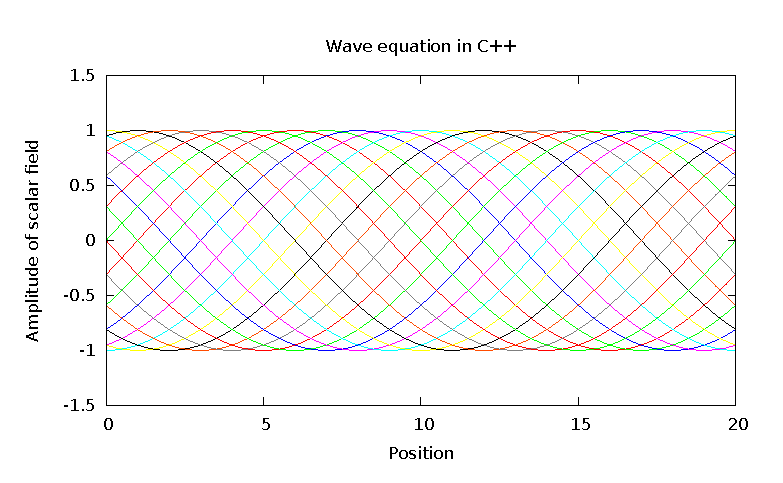
\includegraphics{sineWave}
  \caption{Waves evolving over time for sinusoidal initial conditions}
  \label{sineWave}
\end{figure}

The Discontinuous Galerkin method has truncation error that scales as $h^{n+1}$, where $h$ is the element size and $n$ is the polynomial order of the elements. The $L_2$ error is defined as the square root of the sum of the squared differences across all space, after one complete cycle of the system. Because of the periodic boundary conditions, the system should be the same after one complete cycle, making a meaningful error estimate possible. The scaling of the $L_2$ error with DG order and with element size is shown in Figures~\ref{scalingorder} and~\ref{scalingelement}. The scaling matches expectations until roundoff error is hit, where the error stops improving with order or smaller element size. Not shown, this same pattern was seen for the $L_0$ error, which is the maximum error over all space.

\begin{figure}
  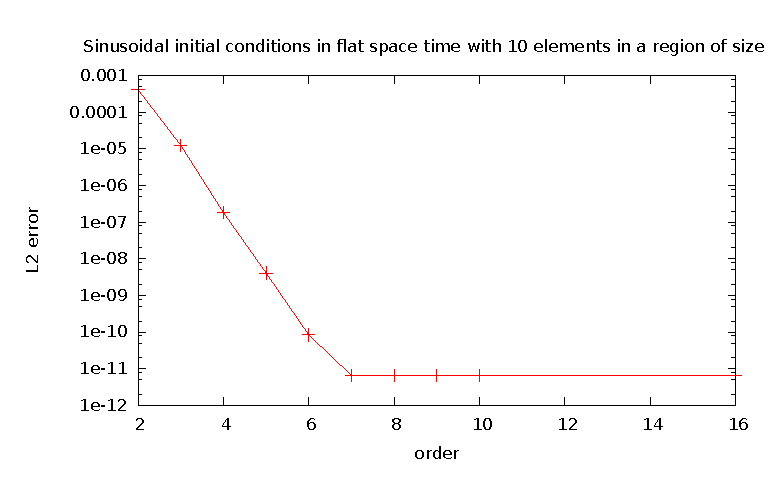
\includegraphics{sinL2WTorder}
  \caption{$L_2$ error scaling with DG order for sinusoidal initial conditions with ten elements with element size $h=0.01$.}
  \label{scalingorder}
\end{figure}

\begin{figure}
  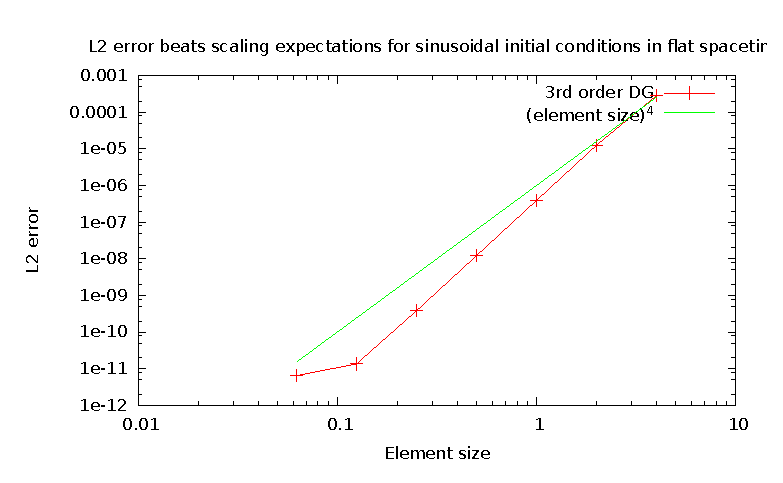
\includegraphics{sinL2WTelement}
  \caption{$L_2$ error scaling with element size for sinusoidal initial conditions. The error seems to be super-convergent. This requires cancellations due to symmetry, perhaps due to the symmetry of wave propagation speed in either direction in flat spacetime.}
  \label{scalingelement}
\end{figure}



\pagebreak
\singlespacing
\chapter{A scalar field on a Schwarzschild background without a source}
\doublespacing
\section{Scalar field on Schwarszchild spacetime}
\subsection{Multipole moment decomposition}
\subsection{Hyperboloidal compactification}
Tortoise coordinates and wave equation
Wave equation in this form
Boundary conditions
\subsection{Initial conditions}
\subsection{final results}


\begin{figure}
  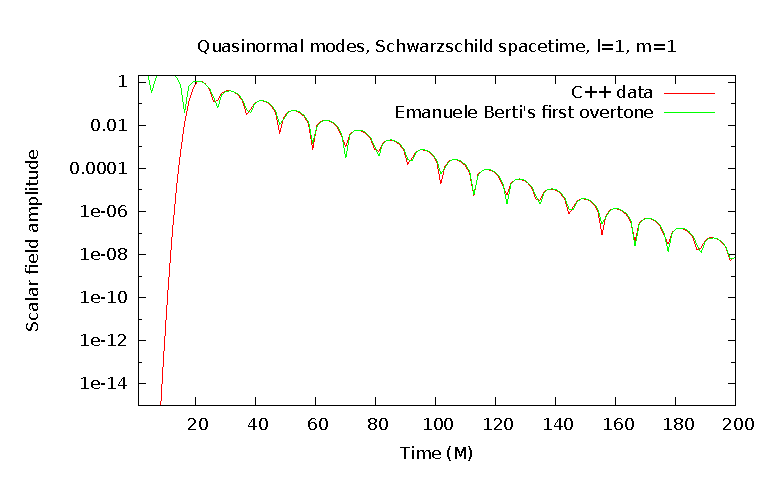
\includegraphics{l1m1qnm}
  \caption{Quasinormal mode for l=1,m=1}
  \end{figure}

\begin{figure}
  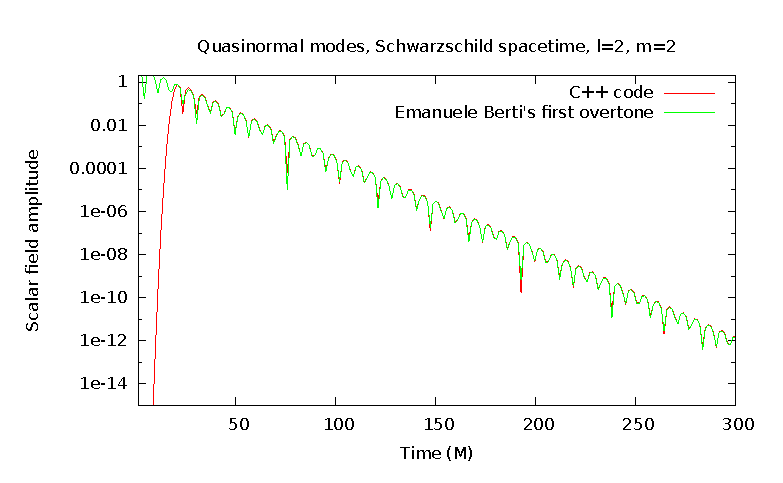
\includegraphics{l2m2qnm}
  \caption{Quasinormal mode for l=2, m=2}
\end{figure}

\begin{figure}
  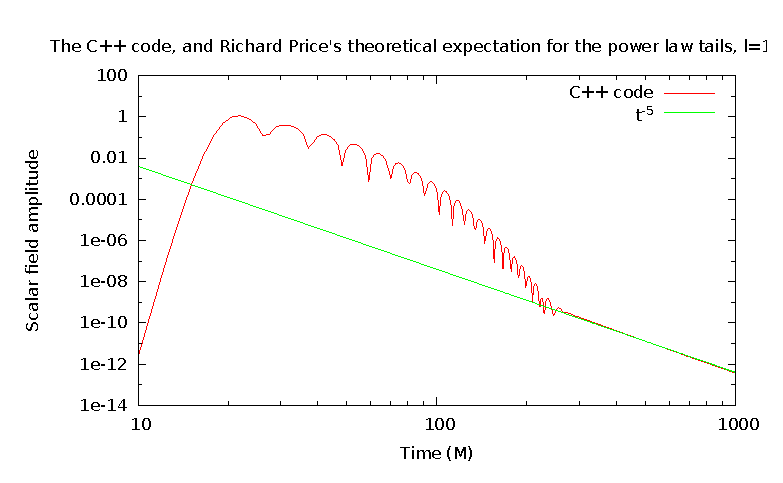
\includegraphics{l1m1tail2}
  \caption{Power law tail, l=1, m=1}
\end{figure}

\begin{figure}
  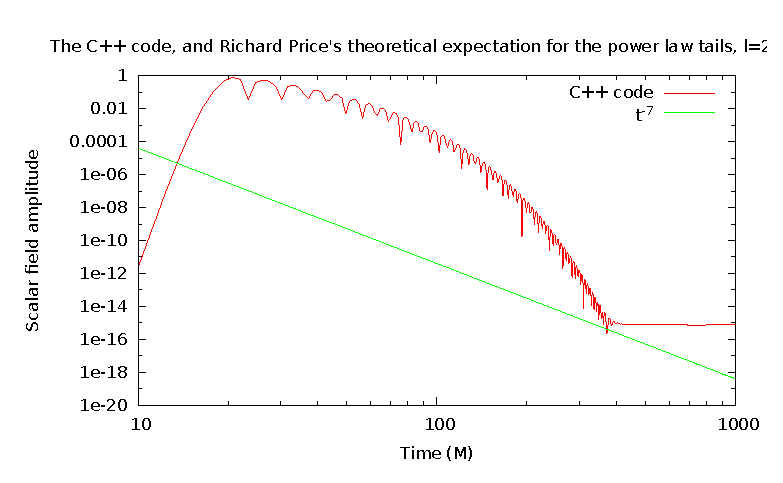
\includegraphics{l2m2tailfail2}
  \caption{Power law tail does not match expectations due to truncation error in DG method, l=2, m=2}
\end{figure}

\begin{figure}
  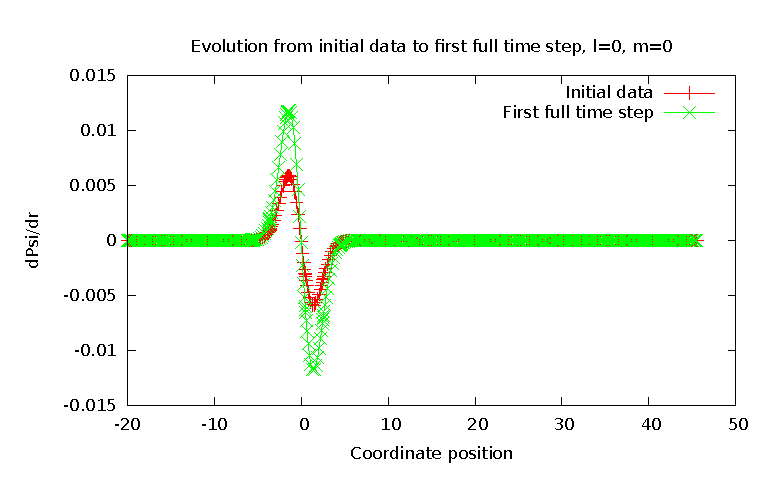
\includegraphics{phi1dl0}
  \caption{Scalar field spatial slice initial condition and first full timestep for l=0.}
\end{figure}

\begin{figure}
  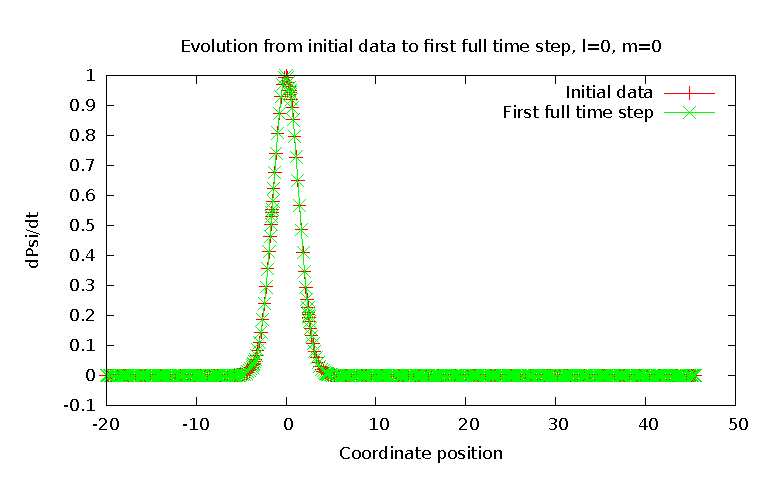
\includegraphics{rho1dl0}
  \caption{Time derivative of the scalar field spatial slice initial condition and first full timestep for l=0.}
\end{figure}

\begin{figure}
  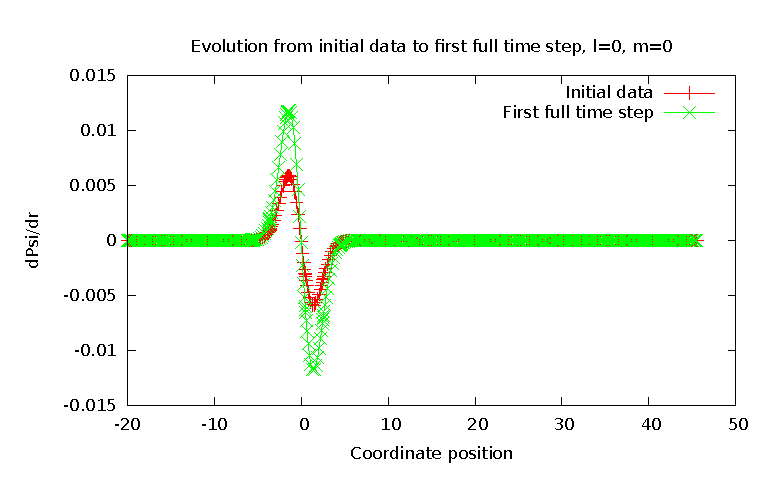
\includegraphics{phi1dl0}
  \caption{Radial derivative of the scalar field spatial slice initial condition and first full timestep for l=0.}
\end{figure}

\pagebreak
\singlespacing
\chapter{Circular orbits on a Schwarzschild spacetime}
\doublespacing


\section{Self Force}

A test particle orbiting a blackhole follows a geodesic, which is the path of extremal proper time. This is described by the geodesic equation,
\begin{equation}
\frac{d^2x^\mu}{d\tau^2}+\Gamma^\mu_{\rho\sigma}\frac{dx^\rho}{d\tau}\frac{dx^\sigma}{d\tau}=0
\end{equation}
where $\tau$ is the proper time and $\Gamma^\mu_{\rho\sigma}$ is the Christoffel symbol, given by~\cite{Carroll}
\begin{equation}
\Gamma^\sigma_{\mu\nu}=\frac{1}{2}g^{\sigma\rho}(\partial_\mu g_{\nu\rho}+\partial_\nu g_{\rho\mu} - \partial_\rho g_{\mu\nu})
\end{equation}

However, a blackhole, of any size, is not a test particle. In the limit of an EMRI, the additional force can be treated perturbatively in the mass ratio of the two particles, in the relativistic case. In the scalar case, the self force is simply written as a delta function source to the wave equation dependent upon the particle's position in time~\cite{WardellSelfForceReview}
\begin{eqnarray}
  \Box\Psi^{ret}=-4\pi q\int\delta_4(x,z(\tau^\prime))d\tau^\prime
\end{eqnarray}
In this equation, $\Box$ is the D'Alembertian and $z(\tau^\prime)$ is the evolving path of the source in spacetime as a function of the particle's proper time. The retarded field $\Psi^{ret}$, is defined to be the field determined by physics taking place at $t_r=t-\frac{|\vec{r}-\vec{r}^\prime|}{c}$; that is, at some distance away from the particle's path, the physical effects of gravity on the scalar field are retarded by light travel time. In the scalar approximation, the particle acts as a delta function point source, with a charge of $q$ and mass $m$. That charge may accelerate or evolve with time; see chapter~\ref{futurework}. 

The retarded field is singular at the location of the particle due to the delta function source. Singularities are computationally problematic. To regularize this singularity, a regular field is created through the use of an effective source.
\begin{eqnarray}
\Psi^R=\Psi^{ret}-\Psi^S\\
\Box\Psi^R=S_{eff}\\
S_{eff}=q\delta(x,x_0)-\Box(W\Psi^S)\\
F_\alpha=(\nabla_\alpha\Psi^r)|_{x=x_0}
\end{eqnarray}
The regularized field, $\Psi^R$, is defined in terms of the retarded field with the singular field, $\Psi^S$, subtracted. This leads to the definition of an effective source, $S_{eff}$, that is zero inside the neighborhood of the particle, due to the world tube window function around the particle, shown in Figure~\ref{wtwindow}, and that approximates the source outside that region. Outside that region, the regularized field is equal to the retarded field. The self-force can be derived from the final equation given above, $F_\alpha$ is merely a gradient of the field itself~\cite{vega_wardell_diener_eff_source}. 


\subsection{World tube}
\begin{figure}
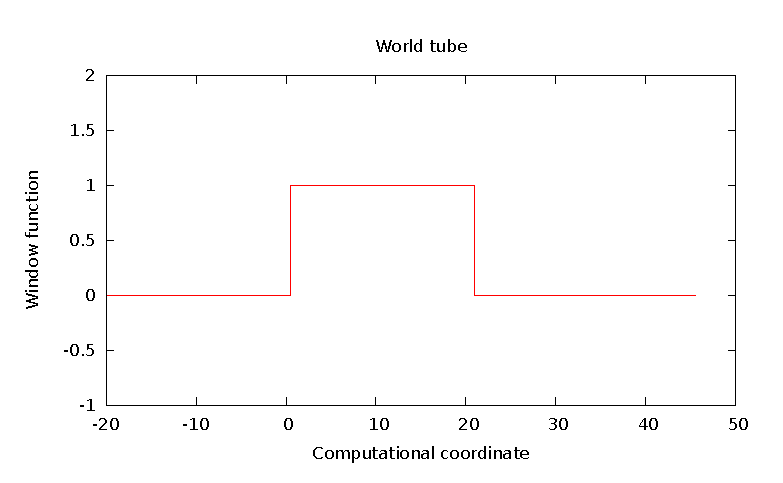
\includegraphics{worldTubeItself}
\caption{Spatial slice of the world tube window function.}
\label{wtwindow}
\end{figure}

The world tube window function around the particle carves out a ring around the blackhole in the orbital plane, due to the use of spherical harmonics to increase the dimensionality of space. In my C++ code, the world tube extends throughout the entire tortoise region, ending at the transitions to the hyperboloidal regions. When calculating numerical fluxes at this boundary, it is necessary to account for both the coordinate transformations between either side of the boundary and the transformation between regular and retarded field.

While on a circular orbit, the particle follows a fixed path that prevents it from inspiraling. This does not conserve energy, since energy is radiated away into the blackhole and to infinity by the scalar waves. Clearly, we are artificially inputting energy into the simulation by holding the particle fixed on its orbit. This, in a nutshell, explains the need for scalar (or gravitational) radiation, and for self force in this limit. 


\section{Comparison between C++ and Fortran codes}

I've performed extensive comparisons between Peter Diener's Fortran code~\ref{heffernan_ottewil_wardell_modesum_basisForCode}, implementing the same thing, and my C++ code. To roundoff precision, they agree, as evidenced by the near-machine-precision ($10^{-15}$) levels of agreement in both absolute and relative error that I achieve in Figures~\ref{circ1},~\ref{circ2},~\ref{circ3}, and~\ref{circ4}

\begin{figure}
  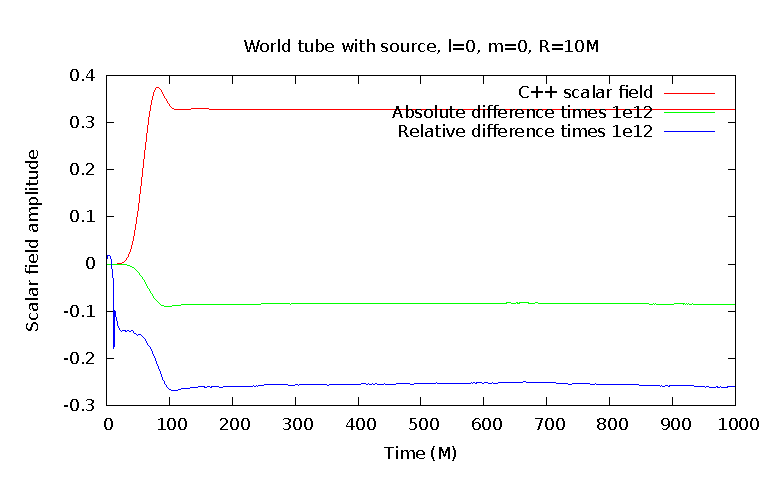
\includegraphics{wtcircl0m0}
  \caption{Comparison between Fortran and C++ codes for a particle on a circular orbit, l=0, m=0.}
  \label{circ1}
\end{figure}
\begin{figure}
  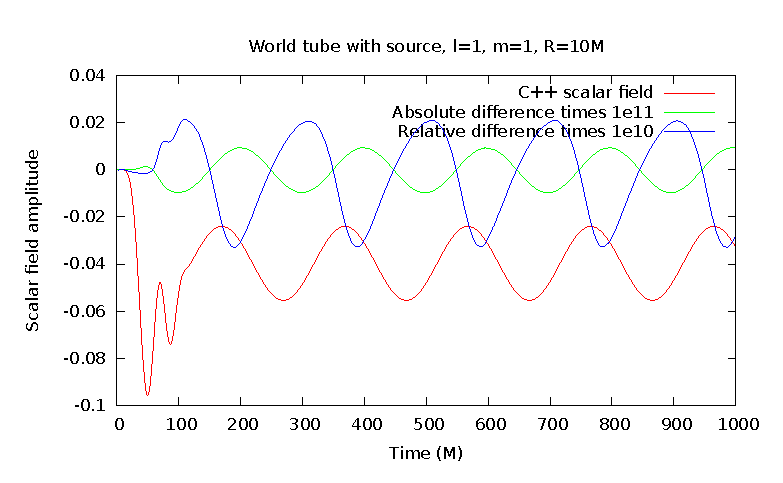
\includegraphics{wtcircl1m1}
  \caption{Comparison between Fortran and C++ codes for a particle on a circular orbit, l=1, m=1.}
  \label{circ2}
\end{figure}
\begin{figure}
  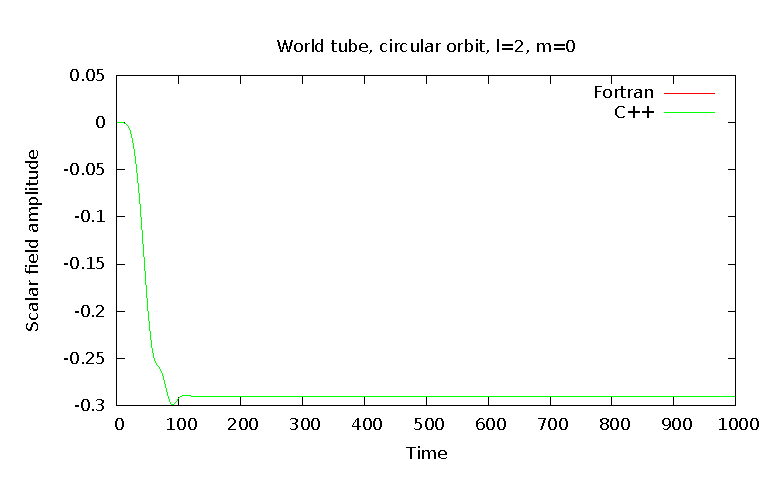
\includegraphics{wtcircl2m0}
  \caption{Comparison between Fortran and C++ codes for a particle on a circular orbit, l=2, m=0.}
  \label{circ3}
\end{figure}
\begin{figure}
  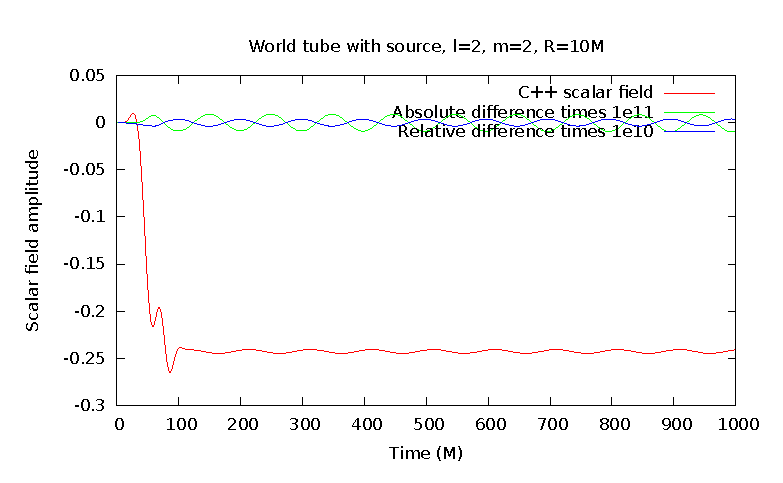
\includegraphics{wtcircl2m2}
  \caption{Comparison between Fortran and C++ codes for a particle on a circular orbit, l=2, m=2.}
  \label{circ4}
\end{figure}

\pagebreak
\singlespacing
\chapter{Elliptical orbits on a Schwarzschild spacetime}
\doublespacing
\begin{figure}
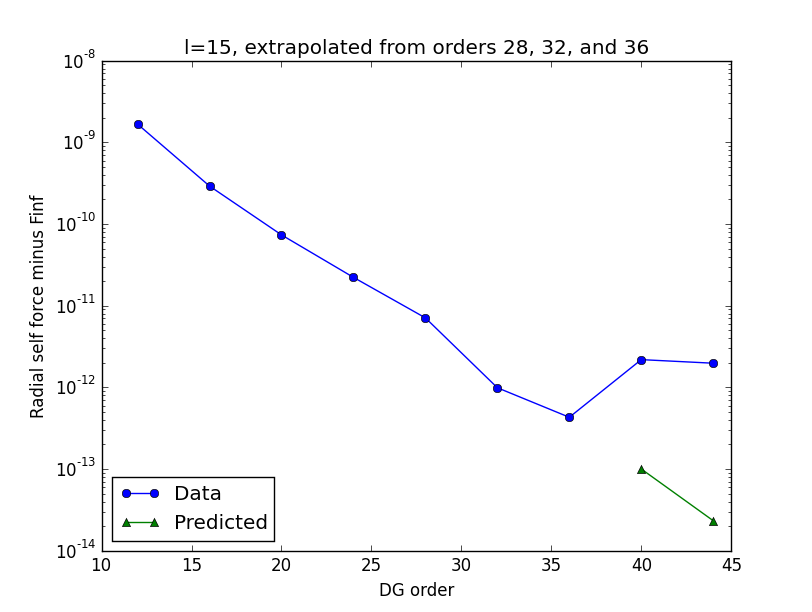
\includegraphics{/home/sdorsher/LabNotebook/20170713/extrapolate7plot}
\end{figure}

\begin{figure}
  \includegraphics{/home/sdorsher/LabNotebook/20170714/finfovertimel3discontinuities}
\end{figure}




t472
\begin{table}
\begin{tabular}{ll}
Starting index & finf\\
2 & 4.18128309016e-05\\
3 & mode failed\\
4 & 4.18128307505e-05\\
5 & 4.18128308245e-05\\
6 & 4.1812830828e-05\\
\end{tabular}
\end{table}


\begin{figure}
  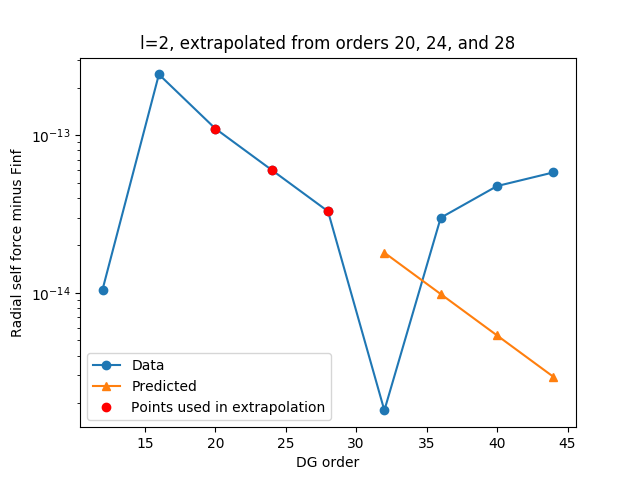
\includegraphics{/home/sdorsher/LabNotebook/20170719/extrapolate7t472l3i2}
\end{figure}

\begin{figure}
  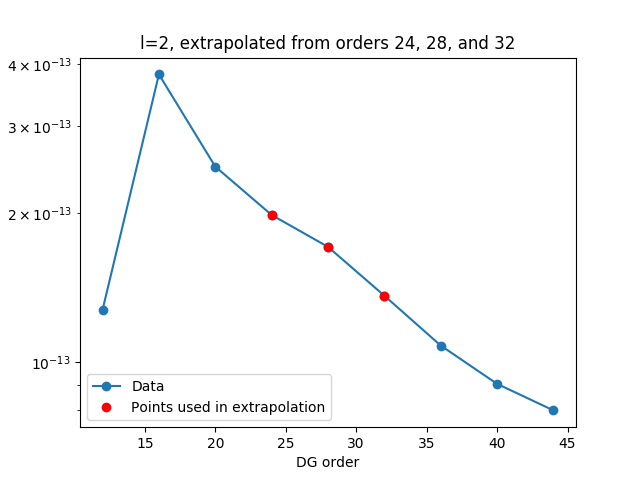
\includegraphics{/home/sdorsher/LabNotebook/20170719/extrapolate7t472l2i3}
  \caption{Note that the three points used in the extrapolation are not on a line on a semilog scale-- it is not possible to fit an exponential through them. That is why this mode failed.}
\end{figure}

\begin{figure}
  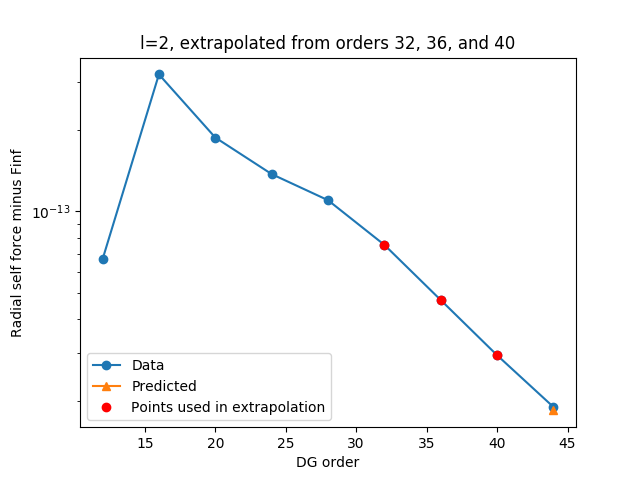
\includegraphics{/home/sdorsher/LabNotebook/20170719/extrapolate7lt472l2i5}
\end{figure}

\begin{figure}
  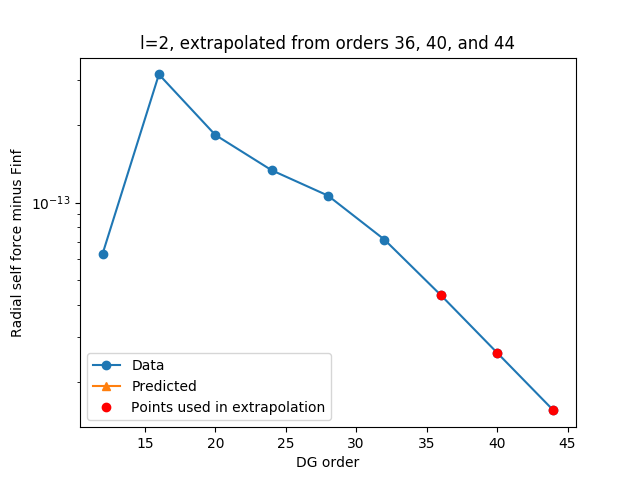
\includegraphics{/home/sdorsher/LabNotebook/20170719/extrapolate7t472l2i6}
\end{figure}

\begin{figure}
  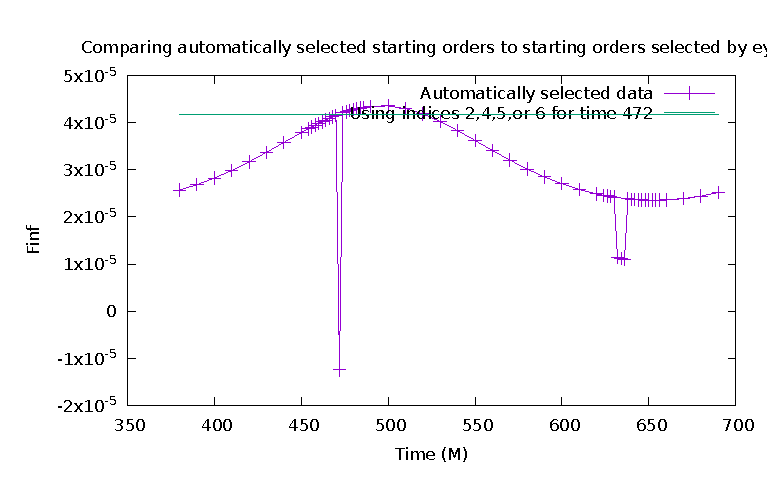
\includegraphics{/home/sdorsher/LabNotebook/20170719/manuallyChosenBestFinft472}
\end{figure}


\section{l=2}
\begin{table}
  \begin{tabular}{lll}
    time & starting order & finf\\
    632 & 0 & mode failed\\
    632 & 1 & 2.40975299617e-05\\
    632 & 2 & 2.40975300465e-05\\
    632 & 3 & 2.40975300114e-05\\
    632 & 4 & mode failed\\
    632 & 5 & 2.40975299291e-05\\
    632 & 6 & 2.40975299148e-05\\
    \hline
    634 & 0 & mode failed (however, 6 selected)\\
    634 & 1 & 2.39990698129e-05\\
    634 & 2 & 2.39990699318e-05\\
    634 & 3 & 2.39990698774e-05\\
    634 & 4 & mode failed\\
    634 & 5 & 2.39990697065e-05\\
    634 & 6 & 2.39990696758e-05\\
    \hline
    636 & 0 & mode failed (however, 6 selected)\\
    636 & 1 & 2.391047416e-05\\
    636 & 2 & 2.39104742806e-05\\
    636 & 3 & 2.39104742249e-05\\
    636 & 4 & 2.39104737911e-05\\
    636 & 5 & 2.39104739924e-05\\
    636 & 6 & 2.39104739079e-05\\
  \end{tabular}
\end{table}

\begin{figure}
  \includegraphics{/home/sdorsher/LabNotebook/20170720/extrapolate7t632l2i1}
\end{figure}

\begin{figure}
  \includegraphics{/home/sdorsher/LabNotebook/20170720/extrapolate7t632l2i2}
\end{figure}

\begin{figure}
  \includegraphics{/home/sdorsher/LabNotebook/20170720/extrapolate7t632l2i3}
\end{figure}

\begin{figure}
  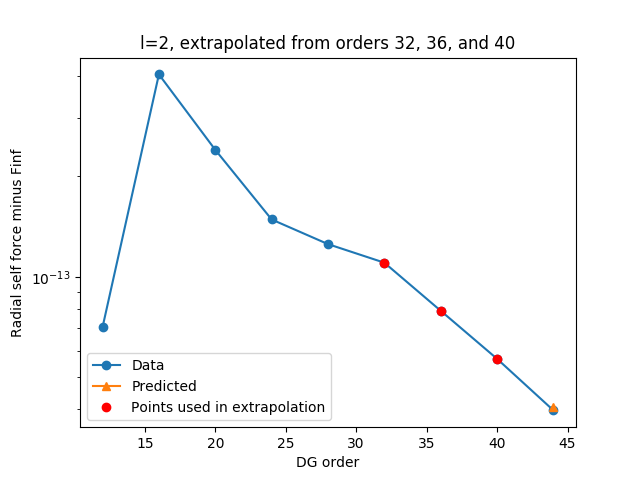
\includegraphics{/home/sdorsher/LabNotebook/20170720/extrapolate7t632l2i5}
\end{figure}

\begin{figure}
  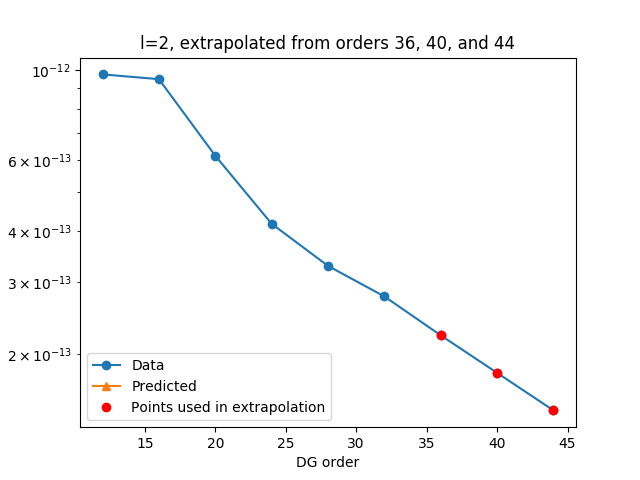
\includegraphics{/home/sdorsher/LabNotebook/20170720/extrapolate7t634l2i6}
\end{figure}

\begin{figure}
  \includegraphics{/home/sdorsher/LabNotebook/20170720/bestFinfManuallyChosent632l2}
\end{figure}

\subsection{ Checking for discontinuities in $F_{\inf}$ for each each l-mode}

There are no discontinuities in $F_{\inf}$ for any of the l-modes when the median approach is used. See mode zero for an example.

\begin{figure}
  \includegraphics{/home/sdorsher/LabNotebook/20170727/finfovertimel0}
  \caption{An example of no discontinuities in $F_{\inf}$ for any of the l-modes. Mode $l=0$.}
\end{figure}


\subsection{Determining $F_{\inf}$ using maximum likelihood fits to subsegments of lines in semilog space}
Fit subsegments of lines in semilog space on DG order convergence plot after subtracting Finf for each possible starting order. pick starting order and starting and ending index of line segment with best possible chi-sq per dof (closest to one). use that finf. veto modes and starting indices that fail the alpha ratio test.

take standard deviation of surface plot as well as average.
\begin{figure}
  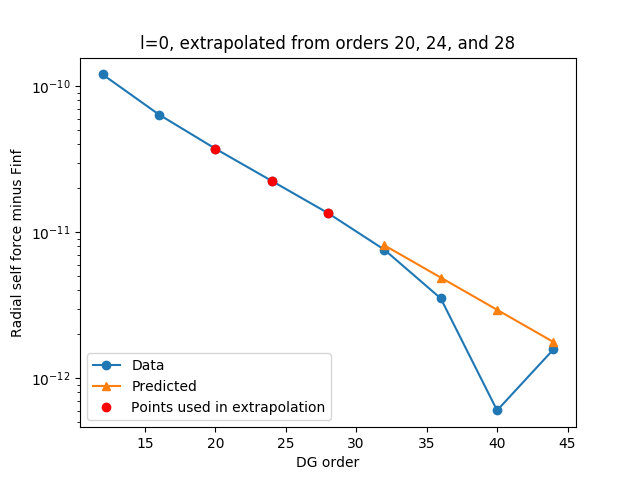
\includegraphics{fittingtechniqet370l0}
  \caption{l=0 mode with fit-chosen starting index produces convergence plot with nice long exponentially converging region}
\end{figure}






\label{ellipticalorb}
\pagebreak
\singlespacing
\chapter{Extrapolating the self force to infinite Disctontinuous Galerkin order}
\doublespacing
To achieve a self-consistent simulation, it is necessary to take the back-reaction into account by evolving the mass and acceleration along with the field itself. The long term goal is to perform an accurate study of the differences between the geodesic evolution method used in Niels Warburton's frequency domain technique and the self-consistent evolution method used in Peter Diener's time domain technique for the scalar approximation to the extreme mass ratio inspiral problem. Diener and Warburton have implemented a preliminary simulation that uses initial conditions from the geodesic case to as a consistency check of the low order modes in the self-consistent simulation. Our simulation has some stability issues that must be addressed to evolve for longer durations. One possible explanation is the truncation error. Another possibility is with the sum of the l-modes. A specific functional form is fit over intermediate values of l to extend the sum analytically past the highest l-mode computed to $l=\infty$. There are uncertainties associated with the manner in which this sum is performed. In this chapter, I explore the truncation error associated with the first order Richardson extrapolation.

\section{First order Richardson extrapolation}

The Discontinuous Galerkin method results in truncation error that scales as $h^{N+1}$, where $h$ is the element size and $N$ is the order of the interpolating polynomials within the element.~\cite{dghesthaven} The radial self force is given by the radial derivative of the scalar field, $F_r=\partial_r\Psi$. However, to obtain this quantity, it is necessary to sum the radial derivatives over all $l$ and $m$ modes. Let $F_l=\sum_{m=-l}^l F_{lm}$. Each of these modes, separately, follows the DG convergence scaling laws. It should be possible to extrapolate to infinite DG order based and obtain the first order Richardson extrapolation, $F_{inf}$, which is the self force for a given l-mode at infinite DG order after a single iteration of the extrapolation of the errors. If the Richardson extrapolation were extended to second order, the error of the error may take on a different functional form, and the second order extrapolation may require a different technique; however, I do not perform it because there is too much random noise in the second order error to determine a functional form.

The three-point exponential extrapolation is motivated by our assumption that Discontinuous Galerkin error is one-sided in the truncation error regime-- it is not random; hence, the self force more or less monotonically approaches a limit. In the round-off error regime where the error is random, the self-force is no longer monotonically converging. As long as it is monotonically converging, it can be written in the form of $F_r(n,l)=F_{inf}(l)+c(l)\exp[-\alpha n]$, where $n$ is the DG order. For a given mode, there is a four step procedure for determining the three parameters associated with the Richardson extrapolation. A root finding technique must be used to solve the following system of equations to determine the exponent of the self force. $\alpha$ must be greater than zero, since the self force is converging with DG order. We use the bisection method. 
\begin{eqnarray}
g(\alpha)-P=&0\\
g(\alpha)=&\frac{\exp[\alpha(n_1-n_2)]-1}{-1+\exp[\alpha(n_1-n_3)]}\\
P=&\frac{F_r(n_1,l)-F_r(n_2,l)}{F_r(n_1,l)-F_r(n_3,l)}
\end{eqnarray}
Secondly, the mode-dependent coefficients of the exponent must be determined.
\begin{equation}
c(l)=\frac{F_r(n_1)-F_r(n_2)}{\exp[-\alpha n_1]-\exp[-\alpha n_2]}
\end{equation}
Finally, the first order Richardson extrapolation, the value of the self force at infinite order, to first order in the errors, depends on the l-mode and the time. The time dependence is implicit in the time dependence of $F_r(n_3)$. 
\begin{equation}
F_{inf}(l,t)=F_r(n_3)-c(l)\exp[-\alpha n_3]
\end{equation}

Sometimes there is not a solution due to roundoff noise causing a deviation from the expected exponential behavior. In practice we allow all three parameters to vary with l-mode and time. I use extrapolation starting orders from the set 12, 16, 20, 24, 28, 32, and 36, with additional data at orders 40 and 44 that may be used as points two and three. Sets of three consecutive DG orders on this list were used. In order to use data from several different DG orders, it was necessary to interpolate between the times at which each order was computed to some desired common set of times. Each order uses different time steps for Courant stability, which requires that time steps are less than the wave travel time to the minimum spacing on the grid. Interpolation was performed using a cubic polynomial scheme. 


\section{Choice of starting order}

Some modes fail because roundoff noise causes the data to deviate from exponential convergence, it is not possible to chose the same starting order for the extrapolation for all modes and all times. This can be done manually, but to produce an evolution over the entire time series to investigate the error as a function of time, it is desirable to automate this process.

\subsection{The last non-NaN method}

The first attempt I made to improve the choice of starting order was to chose the highest starting order for which no lower starting order had been unsolvable. Figure~\ref{finfovertimediscont} shows this approach leads to some discontinuities in the time evolution of $F_{inf}$ in some l-modes ($l=3$ is shown). 


\begin{figure}
  \includegraphics{finfovertimel3discontinuities}
  \caption{Starting order was chosen by iterating from the lowest order to the first order for which the starting order had no solution, and choosing the maximum starting order that succeeded. When $F_{inf}$ is evolved over one full orbital cycle, some l-modes shows discontinuities at some times. l=3}
\label{finfovertimediscont}
\end{figure}

\subsubsection{Manually correcting badly selected automatic values}
To address this concern, I examined the choice of starting order more closely for specific times where discontinuities were present. If the DG orders converged perfectly, they would form a line in semi-log space once $F_{inf}$ is subtracted, if it could be subtracted perfectly. See Figure~\ref{goodbehavior} for an example. Some less perfect examples are shown below. This time is particularly bad, which is why it produced the glitch that requires investigation. $l=2$ and $t=632M$, is shown in a Table~\ref{manual}. Figure~\ref{nosoln} shows an example where no solution is found. The roundoff noise is visible in Figure~\ref{roundoff} at high DG orders. In Figure~\ref{offset}, it is possible the effect at high DG orders is roundoff noise in the $F_r(n,l)$ values of the points, but it is more likely that it is roundoff noise in the choice of $F_{inf}$ due to limitations of the root finding method, resulting in an incorrect offset of the curve. Figure~\ref{manualfix} shows that after selecting an average of the reasonably similar values from Table~\ref{manual}, the discontinuity in the $l=2$ $t=632M$ radial self-force becomes smooth. 


\begin{table}
  \begin{tabular}{ll}
    Starting Order & $F_{inf}$\\
    12 & no solution\\
    16 & 2.40975299617e-05\\
    20 & 2.40975300465e-05\\
    24 & 2.40975300114e-05\\
    28 & no solution\\
    32 & 2.40975299291e-05\\
    36 & 2.40975299148e-05\\
  \end{tabular}
  \caption{Manual starting indices and $F_{inf}$ values for t=632, l=2.}
  \label{manual}
\end{table}

\begin{figure}
  \includegraphics{extrapolate7t632l2i1}
  \caption{Radial self-force with $F_{inf}$ subtracted. Fluctuation in one of the points chosen in the extrapolation, due to roundoff or truncation error, causes the extrapolation to predict a value of $F_{inf}$ that is subtly wrong, leading to curvature in the semi-log plot after $F_{inf}$ subtraction. t=632, l=2, starting order 16}
  \label{nosoln}
\end{figure}

\begin{figure}
  \includegraphics{extrapolate7t632l2i2}
  \caption{Roundoff error is visible at high DG orders. t=632, l=2, i=2}
  \label{roundoff}
\end{figure}

\begin{figure}
  \includegraphics{extrapolate7t632l2i3}
  \caption{Radial self-force with $F_{inf}$ subtracted. The incorrect value of $F_{inf}$ has been chosen due to roundoff error, perhaps due to finite precision in the root finding algorithm, leading to a negative values, that show as a ``V'' in the semi-log plot. t=632, l=2, starting order 24}
  \label{offset}
\end{figure}


\begin{figure}
  \includegraphics{bestFinfManuallyChosent632l2}
\caption{$F_{inf}$ as a function of time. Manual correction for discontinuities in the l=2 mode, using the manually determined $F_{inf}$ data from Table~\ref{manual}. }
\label{manualfix}          
\end{figure}

\subsection{The median method}

To resolve the discontinuity problem, I attempted another approach. I ordered the starting orders that had a solution at each time and for each mode by their $F_{inf}$ values. The median value of $F_{inf}$ was selected, in the hope that it will discard those effected by roundoff and those effected by failure to converge. However, there is no guarantee that it selects those in this regime, since in principle a mode could both be in the roundoff limit and have not converged yet. Yet when this is done, there are no discontinuities in $F_{inf}$ for any of the l-modes when the median approach is used. See mode zero for an example..

\begin{figure}
  \includegraphics{finfovertimel0}
  \caption{An example of no discontinuities in $F_{inf}$ for any of the l-modes. Mode $l=0$.}
\end{figure}


\subsection{The fit method}
A better motivated approach, is to fit subsegments of lines in semi-log space on the DG order convergence plot, and find the longest and most linear region. A fit with the ``best'' value of the reduced chi squared should be a good approximation to this. The reduced chi squared is the value of the sum of the residuals of the fit squared divided by the number of degrees of freedom, which in this case is the number of points in the fit minus two, since there are two degrees of freedom in a linear fit. The expectation value of the reduced chi squared, in the limit of a large number of degrees of freedom, is one. I loop over starting and ending points of the fit, and over starting orders, and choose the starting order with the best fit line segment in the sense that that line segment has a reduced chi squared closest to one. An example of such an automatically chosen starting index is given in Figure~\ref{autoconverge}, where there is a long exponentially converging region. Figure~\ref{abserrfitmedian} shows that the absolute error between fit and median techniques increases with l-mode, possibly indicating that roundoff error becomes a more significant factor in the median technique as the l-mode increases, and the fit technique becomes more important. 

\begin{figure}
  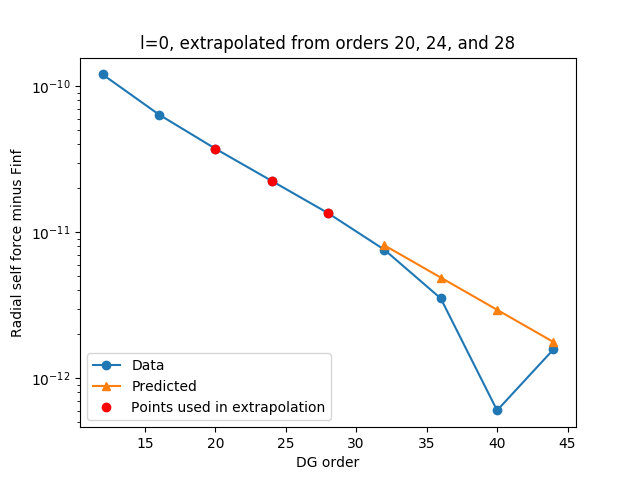
\includegraphics{fittingtechniqet370l0}
  \caption{l=0 mode with line-segment fit-chosen starting order produces convergence plot with long exponentially converging region}
  \label{goodbehavior}
\end{figure}

The absolute error between the fit and median methods increases with l-mode suggesting that roundoff error becomes more important at higher l-modes.

\begin{figure}
  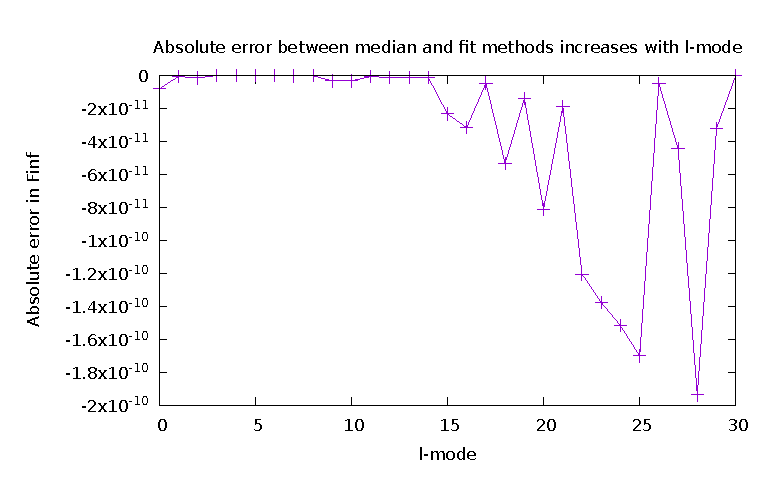
\includegraphics{absErrorIncreaseslmode}
  \caption{Absolute error between fit and median techniques increases with l-mode.}
\end{figure}

There are some outstanding issues with this method. Specifically, I am concerned about the normalization of the the reduced chi-squared, given the unspecified normalization of the second order errors; however, this doesn't seem to prevent the algorithm from nearly working, so perhaps the normalization is nearly correct by chance. Secondly, the fact that the three points used in the extrapolation on the self-force minus $F_{inf}$ curve are precisely on a line in semi-log space means that any hypothesis test is going to be skewed to preferentially select regions including only those three values. To correct for this, it might be better to consider a statistic based upon residuals to the parameters obtained by the extrapolation, with the number of degrees of freedom adjusted to account for the three fixed points. The second order noise is plainly not Gaussian or even unbiasedly distributed, so it is not simple to calculate an expectation value for such a statistic; however, it should have properties similar to the reduced chi squared, so in a back-of-the-envelope sense, can probably be compared to that statistic with the appropriate choice of the degrees of freedom. The biased nature of the second order truncation error is also an issue when using the chi squared test in its usual form. 



\section{The asymptote method}

In a third approach, I consider the behavior of $F_{inf}$ as a function of starting order of the extrapolation. In many, but not all, modes, $F_{inf}$ appears to converge to an asymptote from above or below as the DG starting order increases. However, in many modes, some starting orders produce no solution, so our set of six DG starting orders is reduced to somewhere between three and five. There are two obvious ways to test for convergence: fit an exponent or a power law and do a likelihood ratio test relative to a constant (since the second order errors are unmodelled), or, more reasonably, examine the signs of the first and second numerical derivatives with respect to DG order and consider the end of the convergent regime to be the point where the roundoff noise dominates, and the product of the sign of the derivatives becomes positive. From this derivative sign test, we can determine the best starting order for $F_{inf}$ of a pattern of five or six points that are behaving in a converging like pattern.

However, sometimes, due to high roundoff noise or non-convergent behavior, a low DG order is chosen even for the case where there are five or six good contiguous starting indices. In that case, the asymptotic value of $F_{inf}$ at high DG orders is under-estimated. To achieve a better estimate, I sort this group into the same class as the two, three, and four length contiguous sets of successful DG orders that generated values of $F_{inf}$. For this case, I make an assumption that except for one or maybe two outliers, $F_{inf}$ is approximately constant across the range. The outliers may be at the beginning or the end, or may be due to roundoff noise fluctuations. To reject outliers, I do a standard statistical test of taking the average, making a veto based on the number of standard deviations a point is away from the average, and taking an average again using only the data that survived the veto. I select the point with the value closest to the second average as the best starting order for the extrapolation, and the value I will use to obtain $F_{inf}$. In this case, I found that I got linear curves of $\Psi_r-F_{inf}$ on a semi-log scale for a one sigma veto.

After performing this selection of the best starting order, based on methods to look for asymptotes or reject outliers, I obtained the time evolution of the radial self force, summed from $l=0$ to $l=30$, shown in Figure~\ref{summixed}. The absolute error between $F_{inf}$ and the different DG orders is shown in Figure~\ref{absmixed} and the relative error is shown in Figure~\ref{relmixed}. There is one time where there is some kind of glitch in $F_{inf}$ that remains to be investigated; however, the evolution as a whole appears to be smooth. The absolute and relative error demonstrate that convergence is exponential until about DG order 36 or 40, and which point roundoff noise takes over. The best order for evolutions is therefore DG order 36. The spike is due to $l=25$ at $t=630$, where there is no starting order for which a solution exists. We have examined the time series data and there appears to be some truncation error in mode 16. There also appears to be some roundoff error in $l=25$ at $t=630$, though I have not yet compared it to other times. The truncation error in $l=16$ does not explain the lack of solutions in the extrapolations starting from higher DG orders. The roundoff noise might provide an explanation for this problem, but needs further investigation. In particular, since in the next chapter I conclude that the maximum l-mode that should be included in the fit is $l=24$, I intend to try summing to $l=24$ instead (though this will take significantly more work to implement). The error due to our inability to use a Richardson extrapolation in real time is at the level of $10^{-4}$.

\begin{figure}
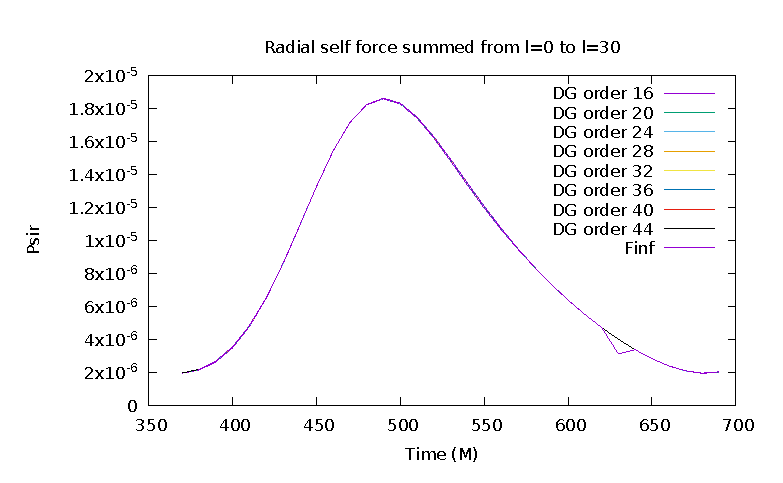
\includegraphics{psirvtwfinfdgorders}
\caption{Sum from $l=0$ to $l=30$ of the radial self force, comparing all DG orders to $F_{inf}$. This was obtained using the method based on asymptotes and averages with rejection of outliers.}
\label{summixed}
\end{figure}

\begin{figure}
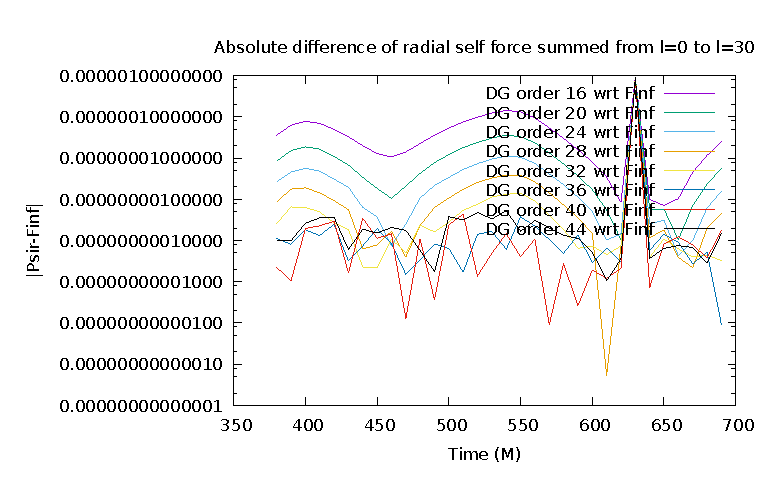
\includegraphics{absdiffpsirvtwfinfdgorders}
\caption{Absolute difference of the radial self force summed from $l=0$ to $l=30$  for each DG order compared to the total radial self force for these modes for $F_{inf}$. This was obtained using the method based on asymptotes and averages with rejection of outliers.}
\label{absmixed}
\end{figure}

\begin{figure}
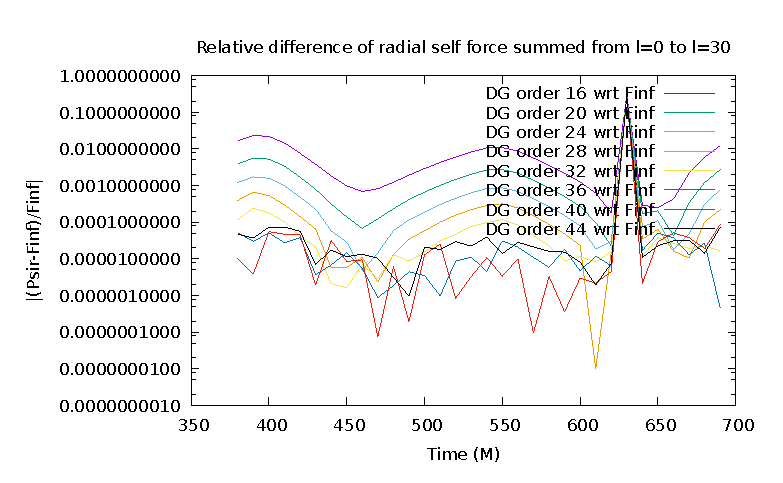
\includegraphics{reldiffpsirvtwfinfdgorders}
\caption{Relative difference of the radial self force summed from $l=0$ to $l=30$  for each DG order compared to the total radial self force for these modes for $F_{inf}$. This was obtained using the method based on asymptotes and averages with rejection of outliers. The error is at the $10^-4$ level.}
\label{relmixed}
\end{figure}

\pagebreak
\singlespacing
\chapter{Extrapolating the mode-summed self-force to include contributions from an infinite number of spherical harmonic modes}
\doublespacing



\subsection{Relative error as a function of mode}
We can understand why it is so hard to produce good fits by examining the relative error between different fitting techniques as a function of mode. Look at the relative error between the fit method and the median method. Both the relative and absolute error grow with l, explaining why the sigma-suppresion technique does not produce good results.

\begin{figure}
  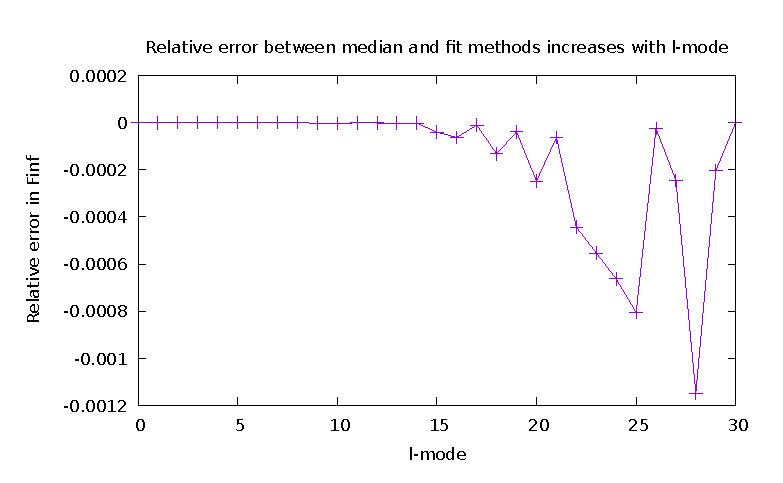
\includegraphics{relErrorIncreaseslMode}
  \caption{Relative error between fit and median techniques increases with l-mode}
\end{figure}


\begin{figure}
  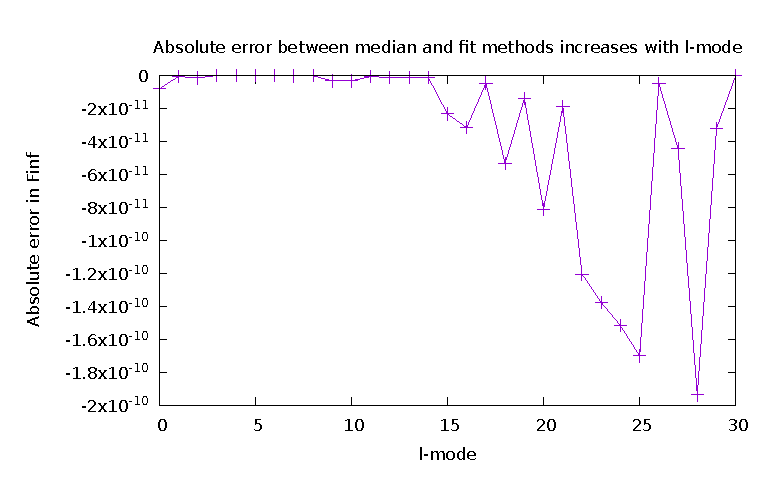
\includegraphics{absErrorIncreaseslmode}
  \caption{Absolute error between fit and median techniques increases with l-mode}
\end{figure}


NEED SOMETHING SHOWING FIT ITSELF. NEED TO REORDER AND RECAPTION NEXT SECTION

\begin{figure}
  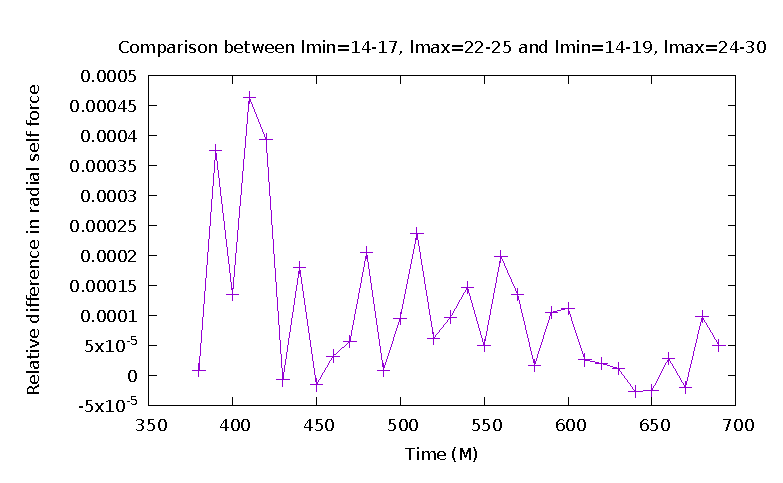
\includegraphics{/home/sdorsher/LabNotebook/20170725/relErrBigSmallRangeOverTime.eps}
  \caption{This is the relative difference between the total radial self force measured in two different ways. In both cases, the self force was extrapolated to infinite order at every l-mode at every possible DG starting order. The infinite DG order self forces over the various starting orders were sorted, eliminating NaNs. The median was chosen for each l-mode. Then the self force as a function of l-mode was fit to its three term form, and the sum was summed from zero to lmax, then extrapolated from $lmax +1 $ to infinity using an analytic form determined using Mathematica. All possible choices with lmin between 14 and 17 and lmax between 22 and 25 were averaged to obtain the total radial self force as a function of time. Similarly, all possible choices with lmin between 14 and 19 and lmax between 24 and 30 were averaged to obtain the total radial self force as a function of time. This plot shows the relative difference. I believe the smaller range is in the denominator.}
\end{figure}

\newpage

\begin{figure}
  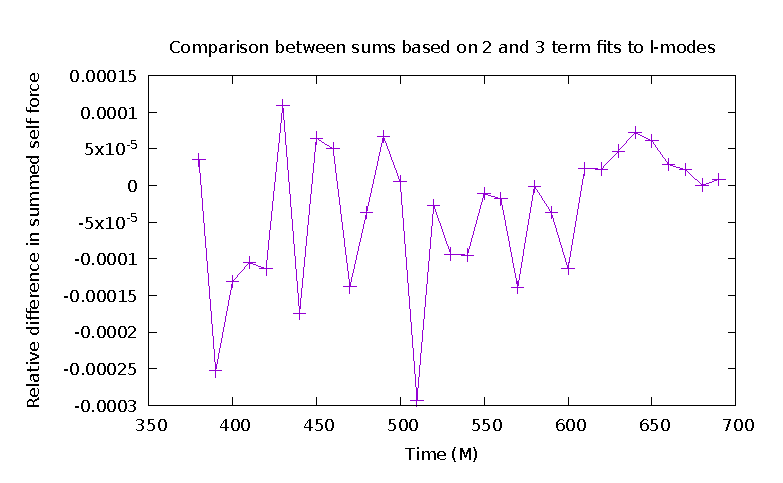
\includegraphics{/home/sdorsher/LabNotebook/20170724/relativeError23termSelfForce.eps}
  \caption{This figure was produced in the same manner as the previous figure, averaging over the smaller range, only it is a comparison between including either two or three terms in the l-mode fit. I believe the three term fit is in the denominator of the relative difference.}
\end{figure}

\begin{figure}
  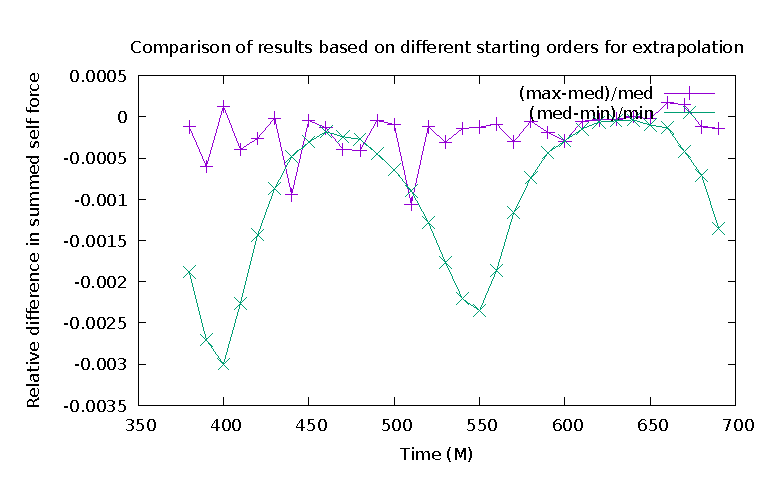
\includegraphics{/home/sdorsher/LabNotebook/20170724/minmaxmedrelativeerror3termavgl.eps}
  \caption{This figure was produced in a similar manner to the first figure, only instead of using the median, it is a comparison between using the median, the maximum, and the minimum. The purple line is the relative difference between the maximum and the median, which is subject to roundoff error due to the potential for the maximum to contian roundoff error. The green line is the relative difference between the median and the minimum, which is subject to effects due to failure to converge. I suspect the median is the best compromise between these two effects, rejecting outliers in both directions, though it is a simplistic approach to doing so, and does not guarantee success. It is possible to have a starting order that has not converged and is also in the roundoff regime, for example. A better guarantee of success, though not a certain one, would be to do a fit over part of the error convergence plot to determine exponentiality, by fitting a line in semilog scale. However, this seems unnecessarily complex at this time.}
\end{figure}
  
\begin{figure}
  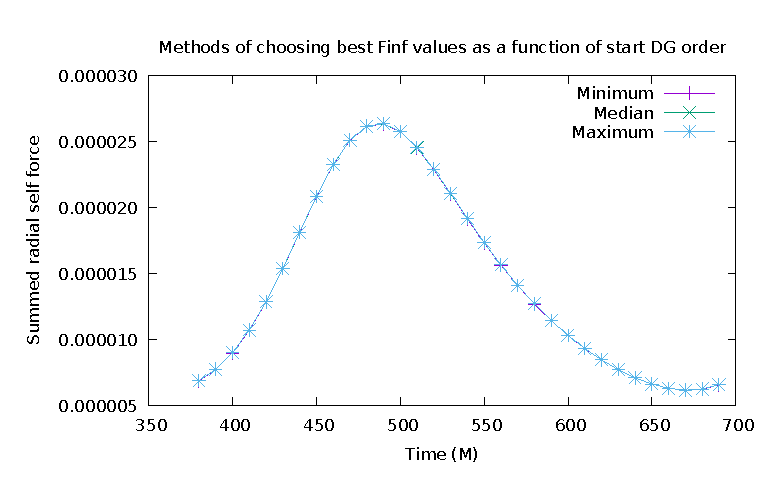
\includegraphics{/home/sdorsher/LabNotebook/20170724/bestfinfscriptplot.eps}
  \caption{This is the actual summed, doubly extrapolated, radial self force, measured in three different ways as described in the three figures above.}
\end{figure}



take standard deviation of surface plot as well as average.


\subsection{Fractional errors}
\begin{figure}
  \includegraphics{fractionalErrorSelfForceOverTime3termMedian}
  \caption{3 term, median method}
\end{figure}

\begin{figure}
  \includegraphics{fractionalErrorOverTimeFits}
  \caption{3 term, fit method}
\end{figure}

\subsection{Structure of the error compared to the evolution in time}
\begin{figure}
  \includegraphics{structErrFitMethod}
  \caption{The structure of the absolute error in comparison to the evolution in time for the fit method}
\end{figure}






\pagebreak
\singlespacing
\chapter{Improving mode fits via a power law scaled weight factor in $\chi^2$ sum}
\doublespacing
\section{Plans for the more distant future}
First, I will update our comparison study with Niels Warburton's geodesic code, to higher l-modes and more recent versions of both codes and report the results to Niels Warburton and Peter Diener.  

I also plan to run Peter Diener's simulation of scalar self-force on a Schwarzschild background for generic orbits including a back-reaction which causes the orbit to evolve away from a geodesic, and examine the data, with the purpose of understanding the physical implications. I will compare Warburton's simulation based on frequency domain initial data and geodesic evolution to Peter Diener's self-consistent time domain code. In the time domain, the state of the field itself naturally accounts for the past orbit of the particle when computing the self force at a given time, assuming sufficient orders of perturbation theory are included. Peter Diener, Ian Vega, Barry Wardell, and Steven Detweiler~\cite{diener_vega_wardell_detweiler_2012} have previously published on self-consistent evolution of a particle around a Schwarzschild black-hole; however, it did not have sufficient accuracy. We are attempting to improve the accuracy using entirely different numerical methods.  in one dimension with spherical harmonics instead of in 1+3 dimensions and using the Discontinuous Galerkin method. 

\section{Self-consistent evolution}
To extend the wave equation to that produced by a particle on a self-consistent orbit, it is necessary to include several additional effects. In addition to the wave equation with a source, the acceleration evolves according to a simplified version of the geodesic equation applied to a scalar particle. The particle also gains or loses mass equal to the work being done on it. 

\begin{eqnarray}
  \Box\Psi^{ret} = -4\pi q \int\delta_4(x,z(\tau^\prime))d\tau^\prime\\
    ma^\alpha=q(g^{\alpha\beta}_{(0)}+u^\alpha u^\beta)\Psi^{R}_{,\beta}\\
    \frac{dm}{d\tau}=-q u^\alpha\Psi^R_{,\alpha}
    \label{genericev}
\end{eqnarray}
The second equation gives the back-reaction due to acceleration of the particle. Here, $\Psi^R$ is the regularized field. The third equation governs the self-consistent evolution of the mass of the particle.~\cite{WardellSelfForceReview}

There are two methods for evolving the orbit that we may use, already implemented in the code by Peter Diener: geodesic evolution and osculating orbits~\cite{pound_poisson}.

\subsection{Geodesic evolution}
The geodesic equation is modified to include a force term on the right hand side in the presence of a self-force or external force~\cite{Carroll}.
\begin{equation}
  \frac{d^2x^\mu}{d\tau^2}+\Gamma^\mu_{\rho\sigma}\frac{dx^\rho}{d\tau}\frac{dx^\sigma}{d\tau}=a^\mu
\end{equation}
This equation, together with Equations~\ref{genericev}, provide the basis for the generic evolution code when the geodesic evolution method is used. 

\subsection{Osculating orbits}

An alternative approach is possible, based upon Reference~\cite{pound_poisson}. In a Schwarzschild spacetime, if the effect of the small black hole is neglected, there is a Killing vector along the time direction and along all three spatial directions, resulting in linear momentum conservation in all directions and hence angular momentum conservation. It is natural to evolve in a physical process that is closely related to these quantities. The eccentric orbit geodesic parameters $p$ and $e$ (semilatus rectum and eccentricity) are chosen (see Chapter~\ref{ellipticalorb} In the self-consistent evolution, the orbit is accelerated from one geodesic to a neighboring geodesic, and gradually evolves through touching geodesics over time. In this process, $p$ and $e$ are updated via a series of ordinary differential equations with extraordinarily complicated right hand sides. This is done using the same RK4 routine that is used to solve the wave equation. It will hopefully be more accurate than the geodesic evolution scheme because angular parameters $\phi$ and $\chi$ monotonically and smoothly increase while $p$ and $e$ evolve slowly, reducing roundoff error. This is in contrast to the accumulation of error introduced through oscillations in $r$ and $t$ in the geodesic method. In the self-consistent approach, the mass and acceleration will also be evolved, eventually. 







\label{sigmachap}
\pagebreak
\singlespacing
\chapter{Future work: generic orbits via the osculating orbits framework}
\doublespacing
\section{plans for the future}
going to test Peter Diener's generic orbits and help him develop them further.

\begin{eqnarray}
  (\Box - \xi R)\Psi^{ret} = -4\pi q \int\delta_4(x,z(\tau^\prime))d\tau^\prime\\
    ma^\alpha=q(g^{\alpha\beta}_{(0)}+u^\alpha u^\beta)\Psi^{R}_{,\beta}\\
    \frac{dm}{d\tau}=-q u^\alpha\Psi^R_{,\alpha}
\end{eqnarray}
R is the Ricci scalar (0 in Schwarzchild spacetime) and $\xi$ is the coupling to curvature. The first equation gives th scalar wave equation in curved spacetime, with a source. The second equation gives the back-reaction due to acceleration of the particle. Here, $\Psi^R$ is the regularized field. The third equation governs the self-consistent evolution of the mass of the particle.~\cite{WardellSelfForceReview}

\section{Generic orbits}
\subsection{Geodesic evolution}
\subsection{Osculating orbits}



\subsection{methods}
effective source
osculating orbits
time dependent coordinate transformation
world tube
already implemented with accelerated orbits though I have not run these.
future work: make self consistent evolution work. 


\pagebreak
\singlespacing
%To insert additional chapters, copy the previous five lines, using chapterX as the argument of the 
%\input command for Chapter X, where X=6,7,8,...
\addtocontents{toc}{\vspace{12pt}}
\addcontentsline{toc}{chapter}{\hspace{-1.6em} REFERENCES}
\begin{thebibliography}{999}
\vspace{0.9em}
\bibitem{formationsmbh}
Volonteri, Marta. (2010). Formation of Supermassive Black Holes. {\em arXiv:1003.4404v1}.

\bibitem{sagastarmultiwavelength}
Yusef-Zadeh, F.; Wardle, M.; Sch\"{o}del, R.; Roberts, D. A.; Cotton, W.; Bushouse, H.; Arendt, R.; Royster, M. (2016). SGR $A^*$ and its environtment: Low-mass star formation, the origin of X-ray gas, and collimated outflow. {\em Astro. Ph. Journal}, 819, 60.

\bibitem{sagastarorbits}
Gillessen, S. ; Eisenhauer, F.; Fritz, T. K.; Bartko, H.; Dodds-Eden, K.; Pfuhl, O.; Genzel, R. (2009). The orbit of the star S2 around SGR $A^*$ from VLT and Keck data. {\em arXiv:0910.3069v1}.

\bibitem{hulsetaylor}
Damour, Thibault. (2015). 1974: the discovery of the first binary pulsar. {\em arXiv:1411.3930v2}.

\bibitem{bmodes}
Guzzetti, M.C.; Bartolo, N.; Liguori, M.; Martarrese, S. (2016). Gravitational waves from inflation. {\em arXiv:1605.01615v3}.

\bibitem{hobbs_dai}
Hobbs, George; Dai, Shi. (2017). A review of pulsar timing array gravitational wave research. {\em arXiv:1707.01615v1}

\bibitem{PriceTails}
Price, Richard H. (1972). Nonspherical Perturbations of Relativistic Gravitational Collapse. I Scalar and Gravitational Perturbations. {\em Phys. Rev. D} 5, 10. 
\bibitem{2ndOrderSource}
Miller, Jeremy; Wardell, Barry; Pound, Adam. (2016). Second-order perturbation theory: the problem of infinite mode coupling. {\em arXiv:1608.0783v1}.

\bibitem{AnnasThesis}
Heffernan, Anna. (2012). The Self-Force Problem: Local Behavior of the Detweiler-Witing Singular Field. University College Dublin. {\em arXiv:1403.6177v1}.

\bibitem{bertiKerrQNM}
Yang, Huan; Zimmerman, Aaron; Zenginoglu, Anil; Zhang, Fan; Berti, Emanuele; Chen, Yanbei. (2013). Quasinormal modes of nearly extremal Kerr spacetimes: spectrum bifurcation and power-law ringdown. {\em arXiv:1307.8086v1}.

\bibitem{bertiSchwQNM}
Berti, Emanuele; Cardoso, Vitor; Starinets, Andrei O. Quasinormal modes of black holes and black branes. {\em arXiv:0905.2975v2}

\bibitem{coordinateTransform}
Philipp, Dennis; Perlick, Volker. (2015). On analytic solutions of wave equations in regular coordinate systems on Schwarzchild background. {\em arXiv:1503.08101v1} 

\bibitem{Detweiler_messaritaki_whiting}
Diaz-Rivera, Luz Maria; Messaritaki, Eirini; Whiting, Bernard F.; Detweiler, Steven. (2004). Scalar field self-force effects on orbits about a Schwarzschild black hole. {\em arXiv:gr-qc/0410011v1}.

\bibitem{diener_vega_wardell_detwieler_2012}
Diener, Peter; Vega, Ian; Wardell, Barry; Detweiler, Steven. Self-consistent orbital evolution of a particle around a Schwarzschild black hole. {\em arXiv:1112.4821v3}.

\bibitem{dirac1938}
Dirac, P. A. M. (1938). Classical theory of radiating electrons. {\em Royal Society Publishing.}

\bibitem{eLISAastrophysicsSelfForce}
Amaro-Seoane, Pau; Gair, Jonathon R.; Pound, Adam; Hughes, Scott A.; Sopuerta, Carlos F. (2014). Research Update on Extreme-Mass-Ratio Inspirals. {\em arXiv:1410.0958v1}.

\bibitem{ELISAz}
Gair, Jonathan R.; Porter, Edward K. (2012). Observing extreme-mass-ratio inspirals with eLISA/NGO. {\em arXiv:1210.8066v1}

\bibitem{gralla_harte_wald_2009}
Gralla, Samuel E.; Harte, Abraham I.; Wald, Robert M. (2009). A Rigorous Derivation of Electromagnetic Self-force. {\em arXiv:0905.2391v2}.

\bibitem{heffernan_ottewil_wardell_modesum_basisForCode}
Heffernan, Anna; Ottewil, Adrian; Wardell, Barry; (2013). High-order expansions of the Detweiler-Whiting singular field in Schwarzschild spacetime. {\em arXiv:1204.0794v4}.

\bibitem{hyperboloidalCoordinates}
Bernuzzi, Sebastiano; Nagar, Alessandro; Zenginoglu, Anil. (2011). Binary black hole coalescence in the large-mass-ratio limit: the hyperboloidal layer method and waveforms at null infinity. {\em arXiv:1107.5402v2}.

\bibitem{LISA02062017}
Danzmann, Karsten. (2017). LISA Laser Interferometer Space Antenna: A proposal in response to the ESA call for L3 mission concepts. 

\bibitem{LISAscienceMarch28_2017}
Babak, Stanislav. (2017). Science with the space-based interferometer LISA. V: Extreme mass-ratio inspirals. {\em arXiv:1703.09722v1}.

\bibitem{miller_wardell_pound_ylm_2ndorder}
Miller, Jeremy; Wardell, Barry; Pound, Adam. (2016). Second-order perturbation theory: the problem of infinte mode coupling. {\em arXiv:1608.06783v1}.

\bibitem{minosasakitanaka}
Mino, Yasushi; Sasaki, Misao; Tanaka, Takahiro. (1996). Gravitational Radiation Reaction to a Particle Motion. {\em arXiv:gr-qc/9606018v1}.

\bibitem{OmegaTransferFunction}
Yunes, Nicolas; Wofgang, Tichy; Owen, Benjamin J.; Briigmann, Bernd. (2006). Binary black hole initial data from matched asymptotic expansions. {\em arXiv:gr-qc/0503011v3}.

\bibitem{poisson_pound_vega_living_review}
Poisson, Eric; Pound, Adam; Vega, Ian. (2011). The Motion of Point Particles in Curved Spacetime. {\em arXiv:1102.0529v3}.

\bibitem{pound2ndOrderSelfForce0}
Pound, Adam. (2012). Second-order gravitational self-force. {\em arXiv:1201.5089v2}.

\bibitem{pound2ndOrderSelfForce}
Pound, Adam. (2017). Nonlinear gravitational self-force: second-order equation of motion. {\em arXiv:1703.02836v1}.

\bibitem{pound_poisson}
Pound, Adam; Poisson, Eric. (2008). Osculating orbits in Schwarzschild spacetime, with an application to extreme mass-ratio inspirals. {\em Phys. Rev. D} 77, 044013.

\bibitem{quinn}
Quinn, Theodore, C. (2000). Axiomatic approach to radiation reaction of scalar point particles in curved spacetime. {\em arXiv:qr-qc/0005030v1}.

\bibitem{quinnwald}
Quinn, Theodore C.; Wald, Robert M. An Axiomatic approach to electromagnetic and gravitational radiation reaction of particles in curved spacetime. {\em arXiv:gr-qc/9610053v1}.

\bibitem{time_dependent_coordinate_transformation}
Field, Scott E.; Hesthaven, Jan S.; Lau, Stephen R. Discontinuous Galerkin method for computing gravitational waveforms from extreme mass ratio binaries. {\em arXiv:0902.1287v2}.

\bibitem{tukolsky_hyperboloidal}
Zenginoglu, Anil; Khanna, Gaurav. (2011). Null infinity waveforms from extreme-mass-ratio inspirals in Kerr spacetime. {\em arXiv:1108.1816v2}.

\bibitem{vega_diener_tichy_detweiler}
Vega, Ian; Diener, Peter; Tichy, Wolfgang; Detweiler, Steven. (2009). Self-force with (3+1) codes: a primer for numerical relativists. {\em arXiv:0908.2138v1}.

\bibitem{vega_wardell_diener_2011}
Vega, Ian; Wardell, Barry; Diener, Peter. (2011). Effective source approach to self-force calculations. {\em arXiv:1101.2925v1}.

\bibitem{Vega_wardell_diener_cupp_haas_2013}
Vega, Ian; Wardell, Barry; Diener, Peter; Cupp, Samuel; Haas, Roland. (2013). Scalar self-force for eccentric orbits around a Schwarzschild black hole. {\em arXiv:1307.3476v2}.

\bibitem{vega_wardel_diener_cupp_haas_accelcirc}
Vega, Ian; Wardell, Barry; Diener, Peter; Cupp, Samuel; Hass, Roland. (2013). Scalar self-force for eccentric orbits around a Schwarzschild black hole. {\em arXiv:1307.3476v2}.

\bibitem{WardellSelfForceReview}
Wardell, Barry. (2015). Self-Force: Computational Strategies. {\em arXiv:1501.07322v3}.

\bibitem{wardell_vega_thornburg_diener}
Wardell, Barry; Vega, Ian; Thornburg, Jonathan; Diener, Peter. (2012). Generic effective source for scalar self-force calculations. {\em arXiv:1112.6355v3}.



\bibitem{GW150914}
LIGO Virgo Collaboration. (2016). Observation of Gravitational Waves from a Binary Black Hole Merger. {\em Phys. Rev. Lett.} 116, 061102.

\bibitem{GW151226}
LIGO Virgo Collaboration. (2016). GW151226: Observation of Gravitational Waves from a 22-Solar-Mass Binary Black Hole Coalescence. {\em Phys. Rev. Lett} 116, 241103.
  
\bibitem{GW170104}
  LIGO Virgo Collaboration. (2017). GW120104: Observation of a 50-Solar-Mass Binary Black Hole Coalescence at Redshift 0.2. {\em Phys. Rev. Lett.} 118, 221101.

\bibitem{LIGO1a}
  LIGO Virgo Collaboration. (2016). Observing Gravitational-wave Transient GW150914 with Minimal Assumptions. {\em Phys. Rev. D} 93, 122004.

\bibitem{LIGO1b}
  LIGO Virgo Collaboration. (2016). GW150914: First Results from the Search for Binary Black Hole Coalescence with Advanced LIGO. {\em Phys. Rev. D} 93, 122003.
\bibitem{LIGO1c}
  LIGO Virgo Collaboration. (2016). The Rate of Binary Black Hole Mergers Inferred from Advanced LIGO Observations Surrounding GW150914. {\em Accepted Astrophys. J. Lett}

\bibitem{LIGO1d}
  LIGO Virgo Collaboration. (2016). Astrophysical Implications of the Binary Black-Hole Merger GW150914. {\em Astrophys. J. Lett} 818, L22.

\bibitem{LIGO1e}
  LIGO Virgo Collaboration. (2016). Tests of General Relativity with GW150914. {\em Phys. Rev. Lett.} 116, 221101.
  
\bibitem{LIGO1f}
  LIGO Virgo Collaboration. (2016). GW150914: Implications for the Stochastic Gravitational Wave Background from Binary Black Holes. {\em Phys. Rev. Lett.} 116, 131102.

\bibitem{LIGO1g}
  LIGO Virgo Collaboration. (2016). Calibration of the Advanced LIGO Detectors for the Discovery of the Binary Black-hole Merger GW150914. {\em Submitted to Phys. Rev. D}.

\bibitem{LIGO1h}
  LIGO Virgo Collaboration. (2016). Characterization of Transient Noise in Advanced LIGO Relevant to Gravitational Wave Signal GW150914. {\em Class. Quant. Grav.} 33, 134001.

\bibitem{LIGO1i}
  LIGO Virgo Collaboration and ANTARES and IceCube Collaborations. (2016). High-energy Neutrino Follow-up Search of Gravitational Wave Event GW150914 with ANTARES and IceCube. {\em Phys. Rev. D} 93 122010. 

\bibitem{LIGO1j}
  LIGO Virgo Collaboration. (2016). GW150914: The Advanced LIGO Detectors in the Era of First Discoveries. {\em Phys. Rev. Lett.} 116, 131103.

\bibitem{LIGO1k}
  LIGO Virgo, ASKAP, BOOTES, Dark Energy Survey and Camera, GW-EM, Fermi GBM and LAT, GRAWITA, INTEGRAL, IPTF, InterPlanetary, J-GEM, La Silla-Quest, Liverpool Telescope, LOFAR, MASTER, MAXI, MWA, PAN-STARRS, PESSTO, PI of the Sky, SkyMapper, Swift, TAROT, Zadko, Algerian National Observatory, C2PU, TOROS, and VISTA Collaborations. (2016). Localization and Broadband Follow-up of the Gravitational-wave Transient GW150914. {\em Astrophys. J. Lett.} 826, L13.
  
\bibitem{Bambi2017}
  Bambi, Cosimo. (2017) Testing black hole candidates with electromagnetic radiation. {\em Reviews of Modern Physics} 89.
\bibitem{LIGOsensitivity}
  Martynov, D.V., et al. (2016). Sensitivity of the Advanced LIGO detectors at the beginning of gravitational wave astronomy. {\em Phys. Rev. D} 93, 112004.
\bibitem{PoissonLivingReviews}
  Poisson, Eric; Pound, Adam; Vega, Ian. (2011). The motion of point particles in curved spacetime. {\em Living Reviews in Relativity}. 14, 7. 

\bibitem{dghesthaven}
 Hesthaven, Jan S.; Warburton, Tim. (2008). {\em Nodal Disconintuous Galerkin Methods: Algroithms, Analysis, and Applications.} Springer.

\bibitem{LIGOSaulson}
 Saulson, Peter R. (1994). {\em Fundamentals of Interferometric Gravitational Wave Detectors.} World Scientific Publishing Co.

\bibitem{NRinC++}
 Press, William H.; Teukolsky, Saul A.; Vetterling, William T.; Flannery, Brian P. (2002). {\em Numerical Recipes in C++: The Art of Scientific Computing.} The Press Syndicate of the University of Cambridge.

\bibitem{Mathematica}
 Wolfram, Stephen. (2016). {\em An Elementary Introduction to the Wolfram Language.} Wolfram-Media, inc.

\bibitem{Python}
 Newman, Mark. (2013). {\em Computational Physics.} University of Michigan.

\bibitem{Wald}
Wald, Robert M. (1984). {\em General Relativity.} The University of Chicago.

\bibitem{Carroll}
Carroll, Sean M. (2004). {\em An Introduction ot General Relativity Spacetime and Geometry.} Addison Wesley.

\bibitem{MTW}
Misner, Charles W.; Thorne, Kip S.; Wheeler, John Archibald. (1973). {\em Gravitation.} W. H. Freeeman and Company. 


\end{thebibliography}
%\pagebreak
%\singlespacing
%\addtocontents{toc}{\vspace{12pt} \hspace{-1.8em} APPENDIX \vspace{-1em}}
%\appendix
%\chapter{Title of Appendix A}
%\vspace{0.5em}
%\input{appendixA}
%\pagebreak
%\chapter{Title of Appendix B}
%\vspace{0.5em}
%\input{appendixB}
%\pagebreak
%If you need to insert additional appendices, copy the previous four lines, using appendixY as the
%argument of the \input commnd for Appendix Y, for Y=C,D,E,...

%Finally, the vita section is created and included in the Table of Contents.
\chapter*{Vita}
\doublespacing
\setlength{\parindent}{1.75em}
\vspace{0.2em}
\addtocontents{toc}{\vspace{12pt}}
\addcontentsline{toc}{chapter}{\hspace{-1.5em} VITA}
My past research has been on comet photometry, x-ray bursts, gravitational lensing and cosmology, exoplanets, neutrino oscillations, theoretical particle physics, gravitational waves, and gravity gradient noise. Most of my background is in simulation, whether statistical or theoretical. I think of myself as a computational physicst and a multimessenger astronomer, though I am not sure that term is widely used. What I mean by it is that I have a broad background in particle physics, particle astrophysics, gravitational wave astronomy, and traditional astronomy. If we can consider my various meanderings as one path toward these two goals, I have been walking this path for more than a decade.

Now I am a fourth year graduate student at Louisiana State University, exactly where I intended to be. My coworkers are good friends. I got to perform photometry of exoplanets with a telescope and analyze the data for myself, bringing a previous project full circle. I have worked on LIGO during the time of three detections. I have had the opportunity to begin to learn multiple techniques for speeding up code and measuring that speed up on supercomputers. I have done a little work with databases and and more with numerical algorithms, and learned a couple of new programming languages. I have had the opportunity to continue to contribute to the field of general relativity and participate in a department where my broad background in the connections between various fields of astronomy is valued. I have helped supervise undergraduate research progress and made a lesson plan for and taught a graduate class, once. This document contains the research I have produced in the last three years since I arrived on June 3, 2014 at LSU and began working with Peter Diener. These have been the best three years of my life.

When interpreting the name on this document, please understand that I am female to male transgendered and that my legal name is Susan Elaine Dorsher but that I go by Steven James Dorsher.
\end{document}





